\documentclass[letterpaper]{article}
% \textit{Required Packages}
\usepackage{aaai17}
\usepackage{times}
\usepackage{amsmath}
\usepackage{helvet}
\usepackage{courier}
\setlength{\pdfpagewidth}{8.5in}
\setlength{\pdfpageheight}{11in}
%\usepackage{hyperref}

\usepackage{footnote}
\usepackage{dblfloatfix}
\usepackage{booktabs} 

\usepackage[flushleft]{threeparttable}

\usepackage{graphicx}
\graphicspath{ {images/} }

\usepackage{float}
\usepackage[draft,inline,nomargin]{fixme}


\usepackage{adjustbox}
\usepackage{multirow}

\usepackage[draft]{changes} 
\newcommand{\mustfix}[1]{\fixme{\hl{#1}}}
\newcommand{\pleasenote}[1]{\fxnote{\hl{#1}}}
\newcommand{\hlfixme}[1]{\fixme{\hl{#1}}}
\newcommand{\fabio}[1]{{\textcolor{blue}{fabio: #1}}}
\newcommand{\yy}[1]{{\textcolor{green}{yy: #1}}}
\newcommand{\apu}[1]{{\textcolor{purple}{apu: #1}}}
\newcommand{\pat}[1]{{\textcolor{red}{Pat: #1}}}
\newcommand{\del}[1]{{\textcolor{gray}{#1}}}



%\%\%\%\%\%\%\%\%\%
% \textit{PDFINFO for PDF\LaTeX{}}
% Uncomment and complete the following for metadata (your paper must compile with PDF\LaTeX{})
\pdfinfo{
/Title (When do ideologues talk to each other? Analyzing factors associated with cross-talk between Feminism and Men's Right Subreddits)
/Author (Patrick Shaffer,Sarvothaman Madhavan,Tyler Dell,Chao Ji,Meng Li,Apu Kapadia,Fabio Rojas)
/Keywords (Reddit, Polarization, Boundary Crossing)
}
%\%\%\%\%\%\%\%\%\%
% \textit{Section Numbers}
% Uncomment if you want to use section numbers
% and change the 0 to a 1 or 2
%\setcounter{secnumdepth}{2}
\setlength\titlebox{2.5in}
%\%\%\%\%\%\%\%\%\%
% \textit{Title, Author, and Address Information}
\begin{document}

\title{When do ideologues talk to each other? Analyzing factors associated with cross-talk between Feminism and Men's Rights Subreddits}

%\author{Patrick Shaffer, Sarvothaman Madhavan, Tyler Dell, Chao Ji, Meng Li, Yong-Yeol Ahn, Apu Kapadia\\
%School of Informatics and Computing\\
%Indiana University Bloomington, IN, USA\\
%patshaff@indiana.edu, madhavas@iu.edu, tdell,jic,li545, yyahn, kapadia@indiana.edu\\
%\AND
%Fabio Rojas\\Department of Sociology \\
%Indiana University Bloomington, IN, USA\\
%frojas@indiana.edu\\}

\author{anonymized}
%\%\%\%\%\%\%\%\%\%
% \textit{Body of Paper Begins}

\maketitle
%\pat{fix overfull box in author names- use first initials?}

\begin{abstract}
Although social media enhances communication across geographical and cultural boundaries, it can also exacerbate the formation of isolated ideological communities. To foster healthy discourse, it is critical to understand how and when opposing groups communicate with each other. Motivated by prior studies linking group participation and the tendency to reach out to other groups, this paper \yy{investigates how multiple aspects of activity measures are associated with the behavior of addressing an ideologically opposed group (``cross-talk'').} \yy{the following sounds something too trivial. higher activity -> more likely to cross talk just by pure chance. } \del{tests the hypothesis that addressing an ideologically opposed group (``cross-talk'') is associated with being highly active in social media.} We test this hypothesis with data from over 133,000 users from two ideologically opposed communities --- the subreddits dedicated to Men's Rights and Feminism. For each user, we collect longitudinal data on their activities to predict when they post a comment on  the opposing subreddit. We apply a proportional hazard model to estimate the importance of various activity variables. We also investigate an important consequence of cross-talk: the linguistic drift between cross-posters and their home subreddit. \yy{per my previous comment, just say we need to make people more active is an empty statement. We did not look at whether more interaction (cross talk) can lead to better discourse. we don't know what's in the cross posts. no content analysis right? It may well exacerbate the polarization.} \yy{we need a better argument} Together, these two results depict one possible path for social change on social media. Individual characteristics, such as user activity and network position, encourage movement across boundaries, which then leads to changes in language and discourse. Thus, polarization might be mitigated by encouraging social media users to interact with others online, especially those who already have a history of crossing boundaries.

\end{abstract}

\section{Introduction}

People form groups based on shared interests, values, and social practices~\cite{gerber2010sociology}. Although group memberships provide individuals with the benefits of developing social identities, they can also lead to detrimental behaviors such as group polarization~\cite{tajfel1979individualsandgroups,tajfel1970experiments,tajfel1979integrative}. Furthermore, the boundaries between communities can often be rigid, and individuals often take it upon themselves to create and enforce social norms about who is to be included or excluded from the group~\cite{sherif1961robbers}. The creation and policing of social boundaries has been heavily investigated by social scientists and researchers in social informatics~\cite{lamont2002study}, and there is now a wealth of knowledge and discussion about social boundaries, whether they emerge from ethnic differences, cultural variance, or professional status ~\cite{abbott1988system,wimmer2008elementary,wimmer2013ethnic} 
%(CITES =  Abbott 1990; Wimmer 2008; 2013). \apu{CITES} %\apu{need citations for each topic in this sentence. In general since we say ``heavily studied'' and ``wealth of knowledge'' we need 6--7 citations at least, and not just one.}. 

Traditional studies of groups have identified various behaviors that may result in crossing of boundaries, adoption of innovations, or other brokerage behaviors~\cite{rogers2003diffusion,tilley2005boundsocties}, yet little research has focused on the precursors to this crossing behavior, in particular the emergence of interactions between individuals in one group and an ideologically opposed group. 

In this work, we seek to understand the factors affecting when individuals begin to interact with an ideologically opposed group. The question of when ``cross-talk'' occurs is important because the interaction between polarized groups gives us insight into the factors that encourage individuals to engage with people who may disagree with them, which can lead to a richer understanding of when network positions reinforce cross-group interactions. 

By studying these precursors to cross-group contact, we add to our knowledge of how groups form ties with one another and how cross-group contacts lead to social change. Sometimes, cross-group contacts may be antagonistic, such as when people intentionally post inflammatory material (``trolling'') and reinforce group boundaries~\cite{bergstrom2011don}. In other cases, cross-group interaction may bring two groups together, e.g., when the members of one group might try to be conciliatory to another group~\cite{cehajic2008forgiveandforget}. While this study does not examine the quality of cross-talk (e.g., antagonistic vs. conciliatory), it provides an important contextualization of cross-talk~--- we offer evidence that individual characteristics of social media users and their network position influence the propensity to address the opposing group (or ``outgroup'').

In this paper, we address this issue by presenting a theory of when individuals in one social group begin to interact with their outgroup and we test our hypotheses with data from Reddit, a popular website where people hold discussions on topics of their choice (e.g., basketball or the 2016 U.S. election). We posit that individuals with a high level of participation on social media and those who have many interactions with others are more likely than others to become cross-posters, and study how various aspects of their activities manifest into the cross-talking behavior. We also investigate the consequence of talk across groups. We show that cross-talking behavior is associated with change in their language, away from the language of the user's original home Subreddit. These two findings indicate a two-stage process: heightened online behavior leads to cross-group talk, which is then associated with changed linguistic patterns. \yy{is it something trivial or more than that? You have different audience, topics, etc., thus it is natural to assume that your language is different in a differnet subreddit. Is this more than that? Maybe it's good to clarify this point early. } 

Drawing on prior research on outgroup interaction, we argue that that heightened online participation should be associated with outgroup contacts~\cite{pettigrew1998intergroup}. To test our theory, we examine online participation based on multiple features. First, we examine the frequency and intensity of a user's posts. A user who posts a lot is not only more likely to cross-talk by pure chance, but also to do so because they are more likely to seek out a new audience. Second, we argue that the direction of the communication matters as well. We examine the difference between the comments written by a user and the comments written in response to a user's comments. \yy{in what way? what are the measures (variables) here?} Third, we suggest that contact with individuals who already cross-talk should be associated with an increased likelihood that a user will cross-talk (which may happen as a result of 'contagion' or 'homophily'). 

We test hypotheses drawn from this theory with data from two large ideologically opposed communities on Reddit, the ``Men's Rights'' and ``Feminism'' subreddits. We view this pair of online communities as a valuable example of two groups separated by a strong social boundary. \yy{the following sentence doesn't sound quite right. revise?} These groups are dedicated to discussing two groups, men and women, who are often seen as having conflicting interests. Furthermore, the proponents of each ideological viewpoint often depict the proponents of the other viewpoint as antagonists. Thus, the boundary between men's rights advocates and feminists should be a particularly strong one that is interesting to examine and provides a test of the strength of the factors that may encourage boundary crossing~\cite{menzies2007backlash,messner2000politicsofmasculinities}. %\fabio{pat, add a cite here} \yy{any literature about Feminism and men's right movements?}\pat{done}

%We test these models with data from the main subreddits dedicated to Men's Rights and Feminism. 
We analyze the data in an event history framework\yy{citatin needed}. For each Reddit user, we collected data for every month after they first appear in either subreddit. Then, we estimated the effect of these possibly time-dependent covariates on the probability that the user will begin to post in the other subreddit (e.g., a ``Feminism'' participant posts in ``Men's Rights''). The correlations are estimated using a proportional hazards, or Cox model, which provides an estimate of the multiplicative effect of the covariates on the transition between states (i.e., switch from not cross-talking to the first instance of cross-talk)~\cite{yamaguchi1991eventhistanal}.  We report bivariate models that link a single variable with cross-talk and multivariate models that include control variables. 

Then, we focus on how cross-posters change. We compare the text that cross-posters produce before speaking to the opposite group and after they speak to the opposite group. Literature on outgroup interaction suggests that interactions with out-group members have the potential to change identities and behavior~\cite{brown1999changing}. Consistent with this theory, we find that the language of cross-posters changes after the first cross-post. The comments written \yy{where? the other subreddit or the home subreddit?} after the first cross-post are less similar to the language of the home Reddit than the comments written before cross-posting. 



%People form groups based on shared interests, values, and social practices~\cite{gerber2010sociology}. Although group memberships provide individuals with the benefits of developing social identities, they can also lead to detrimental behaviors such as group polarization~\cite{tajfel1979individualsandgroups,tajfel1970experiments,tajfel1979integrative}. Furthermore, the boundaries between communities can often be rigid, and individuals often take it upon themselves to create and enforce social norms about who is to be included or excluded from the group~\cite{sherif1961robbers}. The creation and policing of social boundaries has been heavily investigated by social scientists and researchers in social informatics~\cite{lamont2002study}, and there is now a wealth of knowledge and discussion about social boundaries, whether they emerge from ethnic differences, cultural variance, or professional status \apu{need citations for each topic in this sentence. In general since we say ``heavily studied'' and ``wealth of knowledge'' we need 6--7 citations at least, and not just one.}. 
%Traditional studies of groups have identified various behaviors that may result in crossing of boundaries, adoption of innovations or other brokerage behaviors~\cite{rogers2003diffusion, tilley2005identityboundariessocties}, yet little research has focused on the precursors to this behavior, in particular the emergence of interactions between individuals in one group and an ideologically opposed group. 
%In this work, we seek to understand the factors affecting when individuals begin to interact with another group, especially an ideologically opposed group. The question of when `cross-talk' occurs is important because the interaction between polarized groups gives us insight into the factors that encourage individuals to engage with people who may disagree with them, which can lead to a richer understanding of when network positions reinforce cross-group interactions. 
%By studying these precursors to cross-group contact, we add to our knowledge of how groups form ties with one another and how cross-group contacts lead to social change. Sometimes, cross-group contacts may be antagonistic, such as when people intentionally post inflammatory material (``trolling'' and reinforcing group boundaries). In other cases, cross-group interaction may bring two groups together. The members of one group might try to be conciliatory to another group~\cite{cehajic2008forgiveandforget}. While this study does not examine the quality of cross-talk (e.g., antagonistic vs. conciliatory), it provides an important contextualization of cross-talk. We offer evidence that individual characteristics of social media users \apu{such as...} and their network position influence the propensity to address their `outgroup', i.e., the group that they do not identify with or are ideologically opposed to.
%We present a theory of when individuals in one social group begin to interact with their outgroup and we test our hypotheses with data from Reddit, a popular website where people hold discussions on topics of their choice (e.g., basketball or the 2016 U.S. election). Our theory posits that the movement across social boundaries reflects three important social processes as described next.\footnote{We note that our theory only addresses the presence of cross-group contact, not the type of contact.}
%First, the more information an individual in an online community provides to readers, the more likely that they will cross-talk to an ideologically opposite group. We suggest that these individuals who provide a lot of information seek contact with others who may be different. Second, individuals are embedded in social networks which may be associated with a propensity to address an ideologically opposite group. \apu{Does this sentence belong in the previous category?: People who generate discussion online might be more likely to seek contacts with the ideologically opposite group.} People who attract discussion, via comments on what they write, might be encouraged to post their ideas to an ideologically opposed group. Thus, we suggest that the in- and out-degree within an online community's communication network will be associated with the propensity for cross-talk. Third, we suggest that cross-talk will be clustered in the social network. That is, those who cross-talk will be associated with others who cross-talk. This may happen because individuals share similar characteristics (homophily) or one cross-talker may directly influence others (contagion).
%We test hypotheses drawn from this theory with data from two large ideologically opposed communities on Reddit, the `Men's Rights' and `Feminism' subreddits. We view this pair of online communities as a valuable example of two groups separated by a strong social boundary. These groups are dedicated to discussing two groups, men and women, who are often seen as having conflicting interests. Furthermore, the proponents of each ideological viewpoint often depict the proponents of the other viewpoint as antagonists. Thus, the boundary between Men's Rights advocates and Feminists should be a particularly strong one that is interesting to examine and provides a test of the strength of the factors that may encourage boundary crossing~\cite{menzies2007backlash,messner2000politicsofmasculinities}. %\fabio{pat, add a cite here} \yy{any literature about Feminism and men's right movements?}\pat{done}
%
%Thus, using data from the `Men's Rights' and `Feminism' subreddits, we test the following hypotheses:
%\begin{itemize}
    %\item \textbf{H1}: The probability that a Reddit user will `cross-talk' or interact with an ideologically opposite group is correlated with their `openness', as measured by the information they reveal about themselves in their profile, the number of posts they write, and the length of their posts.
    %\item \textbf{H2}: The probability that a Reddit user will `cross-talk' or interact with an ideologically opposite subreddit is affected by their `network interactions', as measured by the number of people who comment on their posts and number of other people's posts that they comment on. 
    %\item \textbf{H3}: The probability that a Reddit user will `cross-talk' or interact with an ideologically opposite subreddit is affected by their interactions with other people who have cross-talked in earlier time periods. \apu{Pat: add ``as measured by...'' I presume we mean they have commented or been commented on by people who have cross-talked in the past?}
%\end{itemize}

%\yy{I feel, at this point, that the hypotheses are all confounded with each other and that it is quite tricky to test those.} \fabio{we have controls like account age, also we can do a factor analysis to address who items in the regression group together}
%We test these hypotheses with data from the main subreddits dedicated to Men's Rights and Feminism. We analyze the data in an event history framework: For each reddit user, we collected data for every month after they first appeared in either subreddit. Then, we estimated the effect of these possibly time-dependent covariates on the probability that the user will begin to post in the other subreddit (e.g., a ``Feminism'' participant posts in ``Men's Right's''). The correlations are estimated using a proportional hazards, or Cox, model, which provides an estimate of the multiplicative effect of the covariates on the transition between states (i.e., switch from not cross-talking to the first instance of cross-talk)~\cite{yamaguchi1991eventhistanal}. 
%\fabio{PAT - add cite to Cox 78 or the Yamaguchi book}\pat{done}
%People form groups based on shared interests, values, and social practices~\cite{gerber2010sociology}. Although group memberships provide individuals with the benefits of developing social identities, they can also lead to detrimental behaviors such as group polarization~\cite{tajfel1979individualsandgroups,tajfel1970experiments,tajfel1979integrative}. Furthermore, the boundaries between communities can often be rigid, and individuals often take it upon themselves to create and enforce social norms about who is to be included or excluded from the group~\cite{sherif1961robbers}. The creation and policing of social boundaries has been heavily investigated by social scientists and researchers in social informatics~\cite{lamont2002study}, and there is now a wealth of knowledge and discussion about social boundaries, whether they emerge from ethnic differences, cultural variance, or professional status \apu{need citations for each topic in this sentence. In general since we say ``heavily studied'' and ``wealth of knowledge'' we need 6--7 citations at least, and not just one.}. 
%Traditional studies of groups have identified various behaviors that may result in crossing of boundaries, adoption of innovations or other brokerage behaviors~\cite{rogers2003diffusion, tilley2005identityboundariessocties}, yet little research has focused on the precursors to this behavior, in particular the emergence of interactions between individuals in one group and an ideologically opposed group. 
%In this work, we seek to understand the factors affecting when individuals begin to interact with another group, especially an ideologically opposed group. The question of when `cross-talk' occurs is important because the interaction between polarized groups gives us insight into the factors that encourage individuals to engage with people who may disagree with them, which can lead to a richer understanding of when network positions reinforce cross-group interactions. 
%By studying these precursors to cross-group contact, we add to our knowledge of how groups form ties with one another and how cross-group contacts lead to social change. Sometimes, cross-group contacts may be antagonistic, such as when people intentionally post inflammatory material (``trolling'' and reinforcing group boundaries. In other cases, cross-group interaction may bring two groups together. The members of one group might try to be conciliatory to another group~\cite{cehajic2008forgiveandforget}. While this study does not examine the quality of cross-talk (e.g., antagonistic vs. conciliatory), it provides an important contextualization of cross-talk. We offer evidence that individual characteristics of social media users and their network position influence the propensity to address the ``outgroup''.
%In this paper, we address this issue by presenting a theory of when individuals in one social group begin to interact with their outgroup and we test our hypotheses with data from Reddit, a popular website where people hold discussions on topics of their choice (e.g., basketball or the 2016 election). We posit that individuals with a high level of participation on social media and those who have many interactions with others are more likely than others to become cross-posters. We also investigate a separate, but related, issue, the consequence of talk across groups. We provide evidence that cross-talk is associated with drifting away from the user's original home reddit. These two findings indicates a two stage process: heightened online behavior leads to cross-group talk, which is then associated with changed linguistic patterns. 
%Drawing on prior research on outgroup interaction, we examine different features of online participation. First, we focus on the frequency and intensity of a user's posts. We argue that the amount of communication is associated with cross-talk because those who communicate a great deal might be more likely to seek out new audiences. Second, we argue that the direction of the communication matters as well. We examine the difference between the comments written by a user and the comments written in response to a user's comments.  Third, we suggest that contact with individuals who already cross-talk should be associated with an increased probability that a user will cross-talk, which may happen as a result of contagion or homophily. 
%We test  hypotheses drawn from this theory with data from two large ideologically opposed communities on Reddit, the ``Men's Rights'' and ``Feminism'' subreddits. We view this pair of online communities as a valuable example of two groups separated by a strong social boundary. These groups are dedicated to discussing two groups, men and women, who are often seen as having conflicting interests. Furthermore, the proponents of each ideological viewpoint often depict the proponents of the other viewpoint as antagonists. Thus, the boundary between men's rights advocates and feminists should be a particularly strong one that is interesting to examine and provides a test of the strength of the factors that may encourage boundary crossing~\cite{menzies2007backlash,messner2000politicsofmasculinities}. %\fabio{pat, add a cite here} \yy{any literature about Feminism and men's right movements?}\pat{done}
%We test these models with data from the main subreddits dedicated to Men's Rights and Feminism. We analyze the data in an event history framework: For each reddit user, we collected data for every month after they first appear in either subreddit. Then, we estimated the effect of these possibly time-dependent covariates on the probability that the user will begin to post in the other subreddit (e.g., a ``Feminism'' participant posts in ``men's rights). The correlations are estimated using a proportional hazards, or Cox, model, which provides an estimate of the multiplicative effect of the covariates on the transition between states (i.e., switch from not "cross-talking" to the first instance of "cross-talk")~\cite{yamaguchi1991eventhistanal}.  We report bivariate models that link a single variable with cross-talk and multivariate models that include control variables. 
%Then, we focus on how cross-posters change. We compare the text that cross-posters produce before speaking to the opposite group and after they speak to the opposite group. Literature on outgroup interaction suggests that interactions with out-group members have the potential to change identities and behavior. Consistent with this theory, we find that the language of cross-posters changes after the first cross-post. The comments written after the first cross-post are less similar to the language of the home reddit than the comments written before cross-posting. 


\section{Social Boundaries and Boundary Crossing}
We view cross-group contact as an example of a broader social process~--- the creation, maintenance, and erosion of group boundaries. A basic observation about human beings is that they create groups where people have shared histories, values, and ideologies~\cite{turner1987rediscovering}. Sometimes, there are strong boundaries between groups, which means that individuals are not likely to interact with people from the ``other'' group or anyone from outside the group~\cite{weisel2015groupconflict}. Examples of strong inter-group boundaries include ethnic divisions, religious denominations, and political parties. In each case, there have been times when there was a strong social boundary between groups. For example, political scientists have documented that there are relatively strong boundaries between Democrats and Republicans in the United States Congress, where bipartisanship is now at a historical low point~\cite{andris2015riseofpartisanship}.

\subsection{The Origin and Evolution of the Term `Boundary Crossing'}

The term `boundary crossing' originated from research concerning the sharing of knowledge between disciplines and professions where factors such as professional affiliations and jargon created occupational boundaries~\cite{wenger1998communitiesofpractice}. Later, researchers approached contact between groups using different disciplinary lenses. Psychologists, for example, have studied outgroup interactions and seek to identify the emotional and cognitive factors that are associated with the willingness to participate in or talk to an outgroup. Sociologists have argued that boundary crossing represents an erosion of social divisions. It is argued that, for example, marriage across ethnic groups is an indicator of weak ethnic boundaries~\cite{qian2007social}. Management scholars argue that linking groups through outgroup contact is bridging a structural hole in a firm, which enhances innovation because it creates new flows of information and provides opportunities for combining ideas \cite{burt2004structuralholes}. 

%In our two subreddits, we noted differences in language which may contribute to the boundaries. More importantly, we see a clear delineation of beliefs and ideas about a common topic --- 
%\yy{use three hyphens --- for m-dash. Fix all m-dashes in the paper.}\pat{done}
%men and women. \citeauthor{hara2014frameworkforkowledgesharing} describe this type of boundary as a cognitive boundary that is ``mentally created'' through ``personal beliefs, worldviews and understanding''~\cite{hara2014frameworkforkowledgesharing}.
%\yy{fix all citations; cite like this~\cite{something}. the tilde creates an empty space and attach the citation to the last word.}\pat{done}
\subsection{Relationship to Political Discussions}

The division between Men's Rights and Feminist proponents is an example of political polarization, which is when individuals sort themselves into groups based on ideological or political affiliations. This sort of social boundary has been extensively studied in both social informatics and political science. \citeauthor{adamic2004divided}~(\citeyear{adamic2004divided}) studied the behavior of political bloggers in the context of the 2004 U.S. Presidential Election and found that two groups, Democrats and Republicans, exhibited different behaviors particularly with regards to how they linked to each other's posts~\cite{adamic2004divided}. 
%\fabio{Unless, I'm computing an inner product, I avoid the word orthogonal in print}
Recent work in political science has examined the extent of polarization in different political contexts. For example, multiple studies have found that Congress is polarized in the sense that there is little cooperation between Republican and Democratic legislators~\cite{andris2015riseofpartisanship}. Other studies of public opinion have documented that people with specific opinions are more likely than before to be firmly associated with a single party~\cite{gould2015partyaffilpoliticalbelief}. E.g., pro-life voters are associated with the Republican party at very high rates, while the opposite is true for pro-choice voters who align themselves with the Democratic party~\cite{killian2008abortion}.

% Continuing in the context of politics, ~\citeauthor{abramowitz2008polarization} refuted a previous study's assertion that political polarization resulted in lower voter turnout and found instead that "polarization energizes the electorate and stimulates political participation" ~\cite{abramowitz2008polarization}. \fabio{NOt sure if this passage follows logically}  

Strong political boundaries are also present on social media~\cite{connover2011politicalpoltwitter}. Numerous commentators have lamented the ability of people to create ``bubbles'' online where they speak primarily, or exclusively, to those who believe the same things. It is also observed that people in one political group often view the other group in adversarial terms, which is consistent with~\citeauthor{allport1979natureofprejudice}'s~(\citeyear{allport1979natureofprejudice}) notion of an ``ingroup'' that defines itself in reference to an ``outgroup''. This observation is consistent with the current study, as analyses of the Men's Rights and Feminist movements document how each group views the other as an antagonist~\cite{messner2000politicsofmasculinities,menzies2007backlash}. 

%\fabio{add cites}\pat{done although this is a repeat of previous cites is that ok?}

%each subreddit is the other's out-group~\cite{allport1979natureofprejudice}. ~\citeauthor{guerra2013measureofpolarization} presented a metric which characterizes the polarization of two groups based on a study of their boundaries~\cite{guerra2013measureofpolarization}.

\subsection{The Importance of Crossing Boundaries}
We also view our work as a contribution to the study of how boundaries are crossed. First, the existence of a contact, or interaction, between two groups is an example of an individual bridging a ``structural hole'' in a social network~\cite{burt2004structuralholes,burt2007burtbrokerage}. Creating a connection between two otherwise disconnected groups is associated with creativity and performance~\cite{burt2004structuralholes,burt2007burtbrokerage}. Second, the linking of two groups facilitates the transmission of information between groups. Third, contact between people may, in some cases, result in the changing of opinions or attitudes. Recent work in political psychology suggests that, in some cases, interpersonal contact between people can change political opinions~\cite{broockman2016reducingtransphobia}. Thus, if cross-talk occurs and it results in positive communication, it may contribute to the reduction of political polarization. Therefore, it is important to understand the individual and contextual factors that contribute to communication between groups. In this paper we use the terms ``crosspost'' and ``cross-talk'' to describe the interactions (using comments) between members of our polarized subreddits. A crossposter is a user who has posted in the opposite subreddit.

%\yy{isn't there something called contact hypothesis or something? (contact between groups -> better mutual understanding) oh yes: https://en.wikipedia.org/wiki/Contact_hypothesis} 

\subsection{Theorizing the Factors that Promote Outgroup Interaction and Studying its Consequences}

We rely on prior research to help us develop hypotheses about the cross-talk in social media. First, a number of previous researchers~\cite{bierhoff2002prosocial} have noted that pro-social people tend to engage in outgroup interaction and boundary crossing. That is, those with a large number of interactions tend to be those that cross social boundaries. Second, working across `structural holes' in networks is often associated with individuals who are often high in `status'. For example, demographers have found that high status individuals often `move up' by marrying persons from even higher status ethnic groups (e.g., high socioeconomic status (SES) African Americans are more likely to marry Whites than low SES African Americans~\cite{wimmer2013ethnic}). In social media, this suggests that degree in communication networks might be associated with cross-talk or outgroup interaction.  Third, recent work in cognitive psychology suggests that even the presence of outgroup members disrupts an individual's identification with their own group~\cite{hobson2016mere}). Thus, being confronted with individuals from outgroups and those who cross post should encourage individuals to reach across social divides. These research findings suggest that frequency and intensity of online interactions, network in- and out-degree, and contact with outgroup members and cross-posters should be associated with cross-posting. 

There are many possible consequences of interaction across groups. The previous discussion suggests one consequence that we will focus on in this paper~--- the loosening of ingroup identification. If it is true that cross-talk might interrupt ingroup identification, then we might expect language will become systematically different than the language of their original group (we call this ``linguistic drift''). The contact of cross-posters with a new group will create a systematic change in how people express themselves online.

%\citeauthor{Zsolt2011NetworkEffectsandPersInfluences} studied the diffusion process of an online social network at the individual level and identified ``degree'' and ``clustering'' effects which influence the adoption of a behavior~\cite{Zsolt2011NetworkEffectsandPersInfluences}. Given the strong polarization of the two groups under study, we note that brokerage in the traditional sense may not occur but analogies to diffusion of a behavior still exist.  For example, while a majority of the authors \pat{cite number} we studied posted only in their preferred subreddit, a small number of authors posted in both subreddits. If we treat the behavior to be diffused as interacting (posting comments) with the other subreddit, then the we can still apply some of the established diffusion theories such as found in ~\citeauthor{Zsolt2011NetworkEffectsandPersInfluences}.  One difficulty presented by our data is that we are unable to determine when the members of one group begin to read the comments and posts in the opposite group (lurking); we can only establish an interaction when an author has made a comment. \citeauthor{sun2014understandinglurkers} provides a comprehensive literature review on the topics of lurkers.

%\fabio{sorry to comment the next section out, but I really couldn't follow it at all}\pat{no problem it was rough anyway}
%\citeauthor{deutsch2011handbook} identified the cause of intergroup conflict as containing ``incompatibilities, behaviors and sentiments''~\cite{deutsch2011handbook}.
%\yy{there are a lot of social psychology references about intergroup conflicts, social identity, etc. this part is too thin.}
%Men'sRights and Feminism exhibit characteristics of homophily which reinforces the polarization and strong boundaries between the two subreddits. Our data spans a considerable time frame, from the creation of Reddit through July 2016. Any changes to the community are therefore reflected in the data.  ~\citeauthor{singer2014evolutionofreddit} found that Reddit appears to be transitioning from "the front page of the internet" to a platform that is   "increasingly self-referential community that focuses on and reinforces its own user-generated image- and textual content over external sources"~\cite{singer2014evolutionofreddit}. \citeauthor{kim2011socialnetworkspoliticaldifferences} found that the use of social networks can lead to exposure to "dissimilar political views"~\cite{kim2011socialnetworkspoliticaldifferences}.  We also note that the authors of the comments under study are anonymous or at least pseudonymous and may use boundary regulation behaviors such as multiple profiles described in ~\cite{stutzman2012boundaryregulation} or may not even be human (bots).

%\citeauthor{currarini2009economicmodeloffriendship} provides detailed background concerning homophily of social groups and the relationship of homophily to group size. The two subreddits observed in this paper differ in size; Men'sRights having considerably more active authors than Feminism~\cite{currarini2009economicmodeloffriendship}. 

%\citeauthor{brundidge2010encounteringdifference} describes the concept of \textit{inadvertency} as it relates to polarization, in particular political polarization in which people who seek a heterogeneous social environment are inadvertently exposed to political difference.  While we have not completed a study of the language and type of interaction of the authors who post in both the Men'sRights and Feminsim subreddits, their existence leave open the possibility of a mechanism for inadvertency.

%\subsection{Diffusion and Brokerage}

%\yy{not entirely convinced that we can use the concept of brokerage in the context of polarized groups as mentioned above. }

\section{Background}

Reddit\footnote{http://www.reddit.com/} is a social sharing and topical discussion forum founded in 2005. It is one of the largest online information sharing and discussion forums, with more than 82 billion page views and more than 73 million posts in 2015~\cite{reddit2015Reddit2015}. Reddit consists of numerous ``subreddits,'' each of which is a topical thread or category containing related content. The users who manage, or edit, a subreddit may impose rules about what may be posted.
 
Users can anonymously create an account which allows them to participate in existing subreddits or create new subreddits concerning a topic of their choosing. There is a subreddit for almost any topic: movies, gaming, sports, politics, and so on. Users can subscribe to subreddits that interest them. 

User subreddit activities include submiting URLs, writing posts, and commenting to posts or other comments. Users may signal their approval, or disapproval, of content by up- or down-voting posts or comments. Upvotes move submissions up the page to make them more viewable to other users, and downvotes move them down the page to make them less viewable. Every submission is coupled with a comment section. Users can comment in reply to the original submission or to another user's comment. Comments can also be voted on with upvotes and downvotes. Upvotes also move comments up the comment section, and downvotes move comments down the comment section. If a comment receives too many downvotes, then it is hidden from view, and users must click to see the comment and in some cases, too many downvotes leads to removal. Users are given link `karma' and comment `karma', which measure how well their content is viewed by other users. A user's link and comment karma denotes their total difference of submission and comment upvotes and downvotes.  


%\del{In 2015 Reddit received 82.43 billion page views, 73.15 million submissions, and 725.85 million comments.} 

\subsection{/r/Men'sRights (MR) and /r/Feminism (Fem)}

The two subreddits under study can be found at https://www.reddit.com/r/Men'sRights/ and https://www.reddit.com/r/Feminism/. Each subreddit page contains the number of subscribers, intent of the subreddit, rules and generally some links to introductory material to get any reader up to speed on the subreddit topic. The feminist moderators' goal for the subreddit is to serve as ``a space for discussing and promoting awareness of issues related to equality for women.'' The Men's Rights moderators' intentions are to serve as ``place for those who wish to discuss Men's Rights and the ways said rights are infringed upon.'' Of interest, the Men's Rights subreddit homepage links to an article by A Voice for Men, a Men's Rights advocacy group, titled ``What's the Difference Between the Men's Rights Movement and Feminism''~\cite{white2011differencebetweenMRandFem}. The article claims that between Men's Right's and Feminism ``there can be no common ground.'' The author claims that there can be no common ground until feminists ``first acknowledge that their movement has spread anti-male bigotry throughout western governments''. % Figure \ref{fig:net_diag} depicts the polarization between these two subreddits.

%\begin{figure}[htb]
%    \centering
    %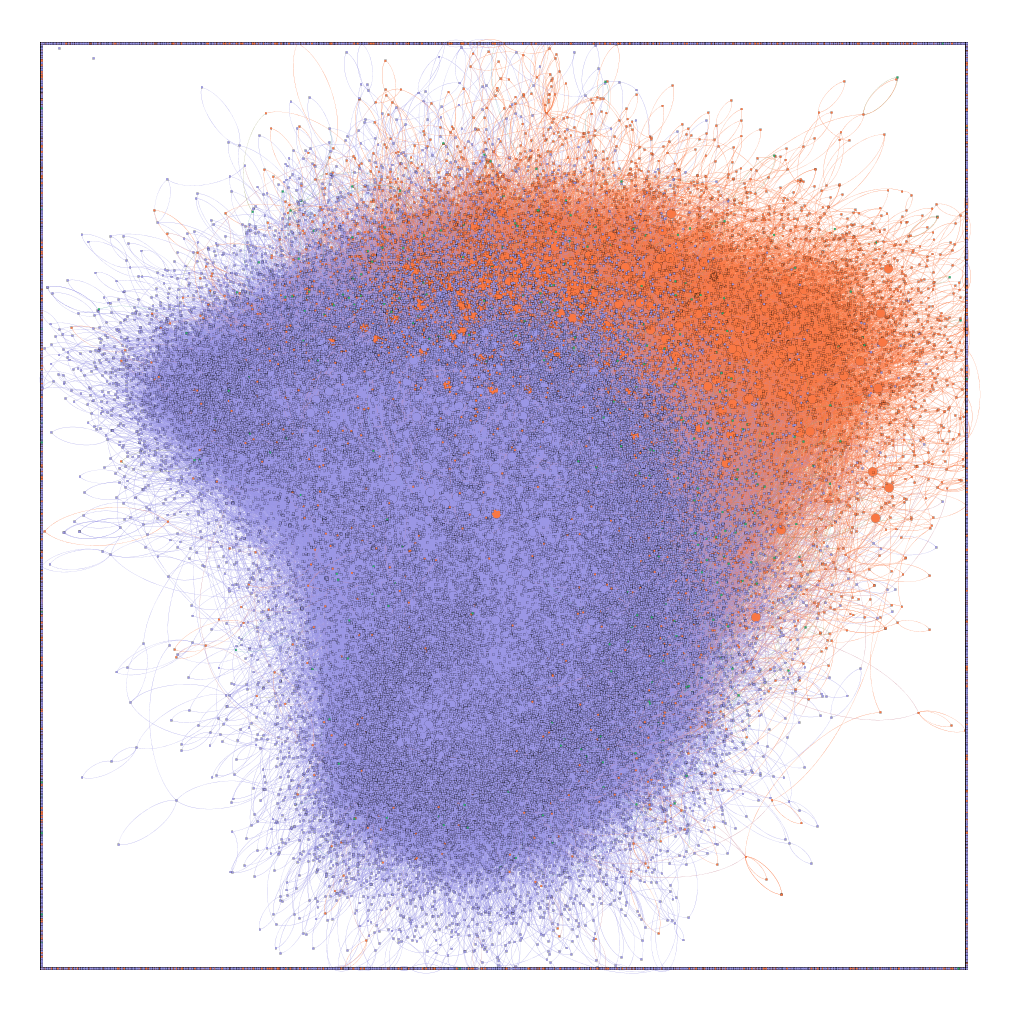
\includegraphics[scale=0.15]{network_dig}
    %\caption{Network Diagram Showing Polarization \yy{it's misleading as the blue nodes and edges block the orange ones. it should be tweaked so that it shows the connection structure better. who drew it? where's the raw file?}}\pat{diagram came from our slack discussions - I'll have to see if the repository contains any better representations}\yy{i remember it's from Meng? I think we should invite her as a coauthor if we were to put a network viz. }
%    \label{fig:net_diag}
%\end{figure}

%\subsection{Interactions Between /r/Men'sRights and /r/Feminism}
% Analysis of authors who post in MR and Fem reveals three distinct groups: authors who post only in MR, authors who post only in Fem and authors who post in both subreddits. Figure \ref{fig:bc_ratio} depicts a timeline of normalized author count by author type. As the larger subreddit, /r/Men'sRights possesses the largest amount of authors, followed by /r/Feminism and finally, authors who comment in both subreddits.  Visualization of comment data in this manner can also lead to other interesting observations, for example the spike in authors who posted in both subreddits during 2012 and 2013 which indicates abnormal rates of intergroup interaction.

\subsection{Data}
The data was retrieved from Google BigQuery and aggregated on https://www.pushshift.io/. %BigQuery is a restful web service for big datasets that works in conjunction with Google Storage launched in May of 2010. BigQuery hosts Reddit comment data. The data set begins in 2005 and is updated to the present. 
As of July 2016, there were over 1.4 billion total comments in the reddit comment dataset.
Table~\ref{tab:datasum} summarizes the comment data after cleaning.


\begin{table}[htb]
    \centering
    \caption{Reddit Commment Data Summary                      }
    \resizebox{\columnwidth}{!}{ 
    \begin{tabular}{|c|c|c|c|c|}
    \hline
    Subreddit & Start Date& Stop Date& \# of Authors&\# of Comments  \\
    \hline
    \hline
    /r/Feminism& 1/11/2009&7/31/2016&31,772&213,082\\
    /r/Men'sRights&3/21/2008&7/31/2016&115,073&2,452,442\\
    \hline
    total&&&146,845&2,665,524\\
    \hline
    \end{tabular}}
    \label{tab:datasum}
\end{table}
 
Because we are focusing on users, we only use comments that are associated with known authors. Comments may not have an associated author if the original author deleted their account. Such comments were removed from the dataset.

%\del{Prior to analysis, the comment data set was cleaned and reduced in size by removing comments where the author had been deleted.  Author deletion in Reddit can occur when the user deletes their account after a comment has been posted. While the comments retain their unique comment id, the linkage to an author is removed.  Often, the comment body is deleted as well. These comments provide minimal value to our longitudinal study and our analysis benefited from their removal. }

%all comments from users of deleted accounts were removed. Since the authors of these comments are unknown, they were removed from the dataset. 

We removed comments from two well-known bots: \texttt{AutoModerator} and \texttt{OriginalPostSearcher}. AutoModerator is a feature of Reddit that allows moderators to establish rules that are automatically enforced. This bot will leave messages indicating that a user violated the subreddit's rules and the comment or post was deleted. OriginalPostSearcher automatically cites cross-posts (``x-posts'') across reddit. A cross-post is a post in a subreddit that was originally posted in a different subreddit. OriginalPostSearcher will automatically comment a citation of the cross post with a link to the original subreddit, author's page, and the original post. We excluded the content generated by these bots from the analysis. From a total of 3,301,859 total comments in the Men's Rights and Feminism dataset, 636,339 comments  were removed before analysis. %(no author- 634,797, AutoModerator - 1,480, and OriginalPostSearcher - 62 comments). \yy{maybe discuss as a limitation in the discussion}

\section{Model Estimation Strategy and Results}
\yy{I'd just say ``Results'' as the section title}

\subsection{Descriptive Results}

We begin with a qualitative description on three types of users: those who post in Men's Rights or Feminism exclusively and those who have posted in both. Figure~\ref{fig:bc_ratio} shows the proportion of each group over time. \yy{The figure is unclear. is this cumulative or decided each month? a user never disappears?} A few things are apparent. First, the Men's Rights subreddit is much more popular than the Feminism subreddit. Second, the majority of users will post in one subreddit and remain there and this is stable over time \yy{this statement is a bit confusing if the figure is cumulative}. Only about 8\% of users would ever post in the other subreddit. Third, there is some modest variation in time. Around 2012, there was an increase cross-talk between these two groups. \yy{if it's a unfounded claim (although it's something that can be checked), maybe we should not say anything about it..} \del{This may be due to the heightened atmosphere generated by the 2012 U.S. presidential election.}

\begin{figure}[tbph]
    \centering
    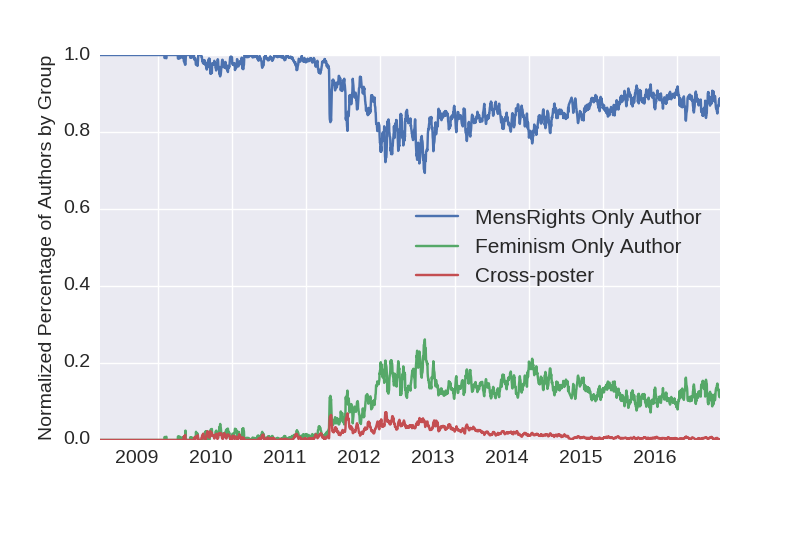
\includegraphics[scale=0.41]{bc_ratios_seabornstyle}
    \caption{Normalized Trajectories of Active Authors by Author Type}
    \label{fig:bc_ratio}
\end{figure}

%\subsection{Statistical Modelling Strategy}
\subsection{Proportional Hazard Model}

Here, we test our hypotheses by applying an event history analysis to a longitudinal data set of user behaviors. For each user, we create time-dependent variables that measure each independent variable over time. \yy{monthly?} The dependent variable is set to zero for all users in the first time period, and switches to one when the user posts to the ``other'' subreddit. That is, if a user first appears in Men's Rights, the dependent variable is zero until they post in Feminism. \yy{one important measurement missing here: to convincingly argue that the home subreddit is really meaningful, we need to show that the first subreddit the users post is what they will post most in the future. among the 8\% of users, in how many users their posting in the first subreddit overwhelmingly dominate their posts? This is critical for arguing that the ``first subreddit'' is meaningful.} Conversely, a user who appears in Feminism has a dependent variable scored as zero until they post in the Men's Rights subreddit. Since we are modelling the one-way transition between states, we do not use data from the period after the first instance of cross-talk. Thus, for most cases, the dependent variable is zero for all time periods because, as Figure \ref{fig:bc_haz} shows, most users never post in the ``other'' subreddit. For approximately 8 percent of cases, the dependent variable will eventually switch to one. Our initial exploration of the data suggested that monthly time periods were appropriate. Most cross-talking starts, if it ever happens, approximately eighteen months after the initial post in the ``first'' subreddit, which suggests that daily or weekly measurements would create zero inflated data and yearly measurements would suppress variation in the time to first cross-talk.

The proportional hazard model is a statistical model of the transition between states. The intuition of the model is that the odds of transitioning between states depends on two things, an underlying hazard rate that varies over time and the effects of the covariates (features). Some variables, like gender, might be fixed while others vary over time, like yearly income. The model estimates a multiplicative effect of the covariates on the rate of transitions. When estimated using maximum partial likelihood estimation, the model produces coefficients that are very similar to a logistic regression model, the coefficients indicate a multiplicative effects on the odds of transition~\cite{blossfeld2014event}. %%% ---- Sarvo added the equation ---- %%%%
The Cox proportional hazard model has the form (at time $t$)\\
\begin{equation}
\begin{split}
\lambda(t | X_{i}) & = \lambda_{0}(t) \exp(\beta_{1}X_{i1}+..+\beta_{p}X_{ip}) \\ 
&= \lambda_{0}(t) \exp (X_{i}^T \beta), 
\end{split}
\end{equation}
where $\lambda$ is a \emph{hazard function}, $X_{i} = (X_{i1},. . ., X_{ip})^T$ is the covariate vector for subject $i$, and $\beta$ is the coefficient vector. 

%%% ---- Sarvo added the equation ---- %%%%

%\del{The main purpose of this paper is to test three hypotheses about the tendency for a Reddit user to begin posting in the ``opposite'' subreddit. The modelling strategy that we employ is event history analysis. That is, we created a longitudinal data set of Reddit users that contains information about the reddit user, their behavior, and when they begin to post in the ``other'' subreddit.} \del{The transition from ``not boundary'' to ``boundary crossing'' is modelled as a discrete event. Thus, the data is organized in a longitudinal matter.} The independent variables may change over time and the dependent variable is equal to zero until the event occurs. In that time period, the dependent variable switches to one. \yy{more precise definitions and proper citations please}

Our independent variables are defined in the following way. First, we produce two measures of openness: the number of characters in the user's account name (which is fixed over time) \yy{needs justification} and the average monthly number of words they write in their ``first'' subreddit (e.g., Men's Rights or Feminism) \yy{again, it's conspicuous here that we don't actually know whether the first subreddit align well with ppl's identity.}. Second, we produce measures of network in- and out-degree. We collect the number of monthly comments they write on other redditors posts (out-degree) and the number of monthly comments made on posts written by the user (in-degree). To assess the degree of clustering among cross-talkers, we measure the monthly number of cross-posters who comment on a user's posts and the monthly number of comments the user leaves on threads started by cross-talkers. 

We include the following control variables in the analysis. First, we include the account age in months to account for the fact that people who have been on Reddit long might be more willing to rech out to different groups. Second, we include a measure of the user's quality of comments by include the average monthly score (up votes minus down votes). This addresses the possibility that cross-posting is associated with people who are more effective communicators. We also include variables that account for the interaction between the user and those from within their subreddit or the opposing subreddit. We also include dummy variables for each subreddit to account for unmeasured user heterogeneity and yearly dummy variables to account for the possibility that the tendency to cross post varies over time.
 
\begin{table}[htb]
    \centering
    \caption{Comment Variables and Descriptions}
    \resizebox{\columnwidth}{!}{ 
    \begin{tabular}{|c|p{6cm}|}
    \hline
    Variable &	Definition\\
    \hline
    \hline
    First Cross-Talk& 1 if the user cross-talked for the first time in current month, 0 else\\
    Name Length& Username Length \\
    %account.post.karma& Total Account post Score\\
    %account.comment.karma& Total Account comment Score\\
    %karma\_ratio& Ratio of Account Score to Comment Score\\
   Account Age& Number of days since account was created\\
    Feminism & 1 if Homesubreddit is Feminism, 0 else\\
    wordiness & number of words per/post in a month \\
    Comments Written by User & number of outgoing comments in a month\\
    Comments on User’s Posts & number of incoming comments in a month\\
    Average Score & Mean score in a month\\
    Crossposter Talks to User & 1 if a crossposter talked to me, 0 else\\
    User Talks to Crossposter & 1 if I talked to a crossposter, 0 else\\
    %other\_sr\_to\_me&	1 if someone from the other subreddit talked to me, 0 otherwise\\
    %me\_to\_other\_srs&	1 if I talked to someone from other subreddit, 0 otherwise\\
    \hline
    \end{tabular}}    
    \label{tab:field_def}
\end{table}

We present the results of the event history analysis in two parts. First, we discuss selected hazard curves, which provide intuition about the effects of the independent variables on the decision to post in the ideologically opposite reddit. A hazard curve visualizes the proportion of people over time who adopt a new behavior. The hazard curves start in the month in which the oldest subreddit began - Feminism - which is labeled ``30'' because thirty months passed since the beginning of reddit. Then, we will present the results of the Cox proportional hazards model.

Figure~\ref{fig:bc_haz} shows the hazard curve by original ``home'' subreddit. \yy{define the hazard rate plz} That is, we look at the hazard rate for the entire population and separately for each subreddit. \yy{unclear how it is aggregated} As suggested by the Figure~\ref{fig:bc_haz}, there is a difference between the two ideological subreddits, with Feminist redditors cross-talking at a higher rate than their counterparts. \yy{I don't think we have evidence to claim this. As I wrote before, it can purely come from the size difference. There can be many null models that may explain this without assuming any systematic differences between participants.} \del{This strongly suggests that there are systematic differences between participants in the Men`s Rights and Feminism reddits.} Figure~\ref{fig:ctc_haz} shows that having contact with a cross poster has a substantial effect on cross posting. \yy{activity-controlled? if not, it may be rather trivial (more activity -> more likely to cross post by pure chance). unclear to me how these curves are obtained. precise definitions are needed. } Figure \ref{fig:outmean_haz}. shows that those who leave comments on other posts are much more likely to post.

\begin{figure}[ht]{}
\centering
    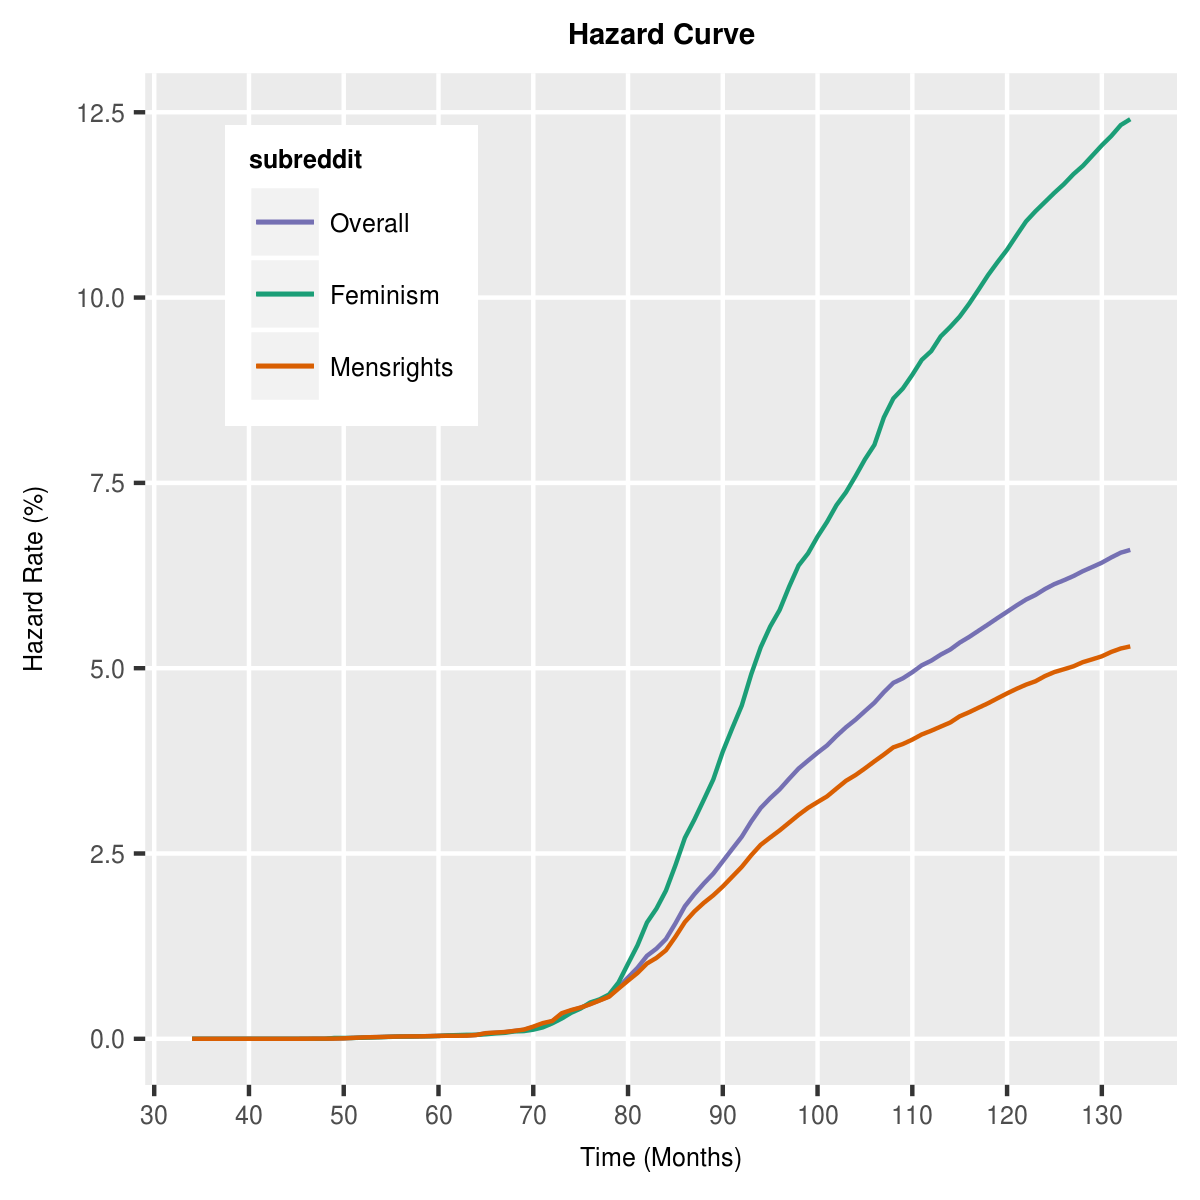
\includegraphics[scale=0.75]{Overall_Hazard_thick}
    \caption{Hazard Curve by Home Subreddit}
    \label{fig:bc_haz}
\end{figure}

%We found other differences. Figure \ref{fig:ctc_haz} shows that there are smaller, modest differences between those individuals who have had contact with other \pat{authors who have posted in the opposite subreddit (``boundary crossers'')} \del{boundary crossers} when compared to those who have not had contact.

\begin{figure}[ht]{}
\centering
    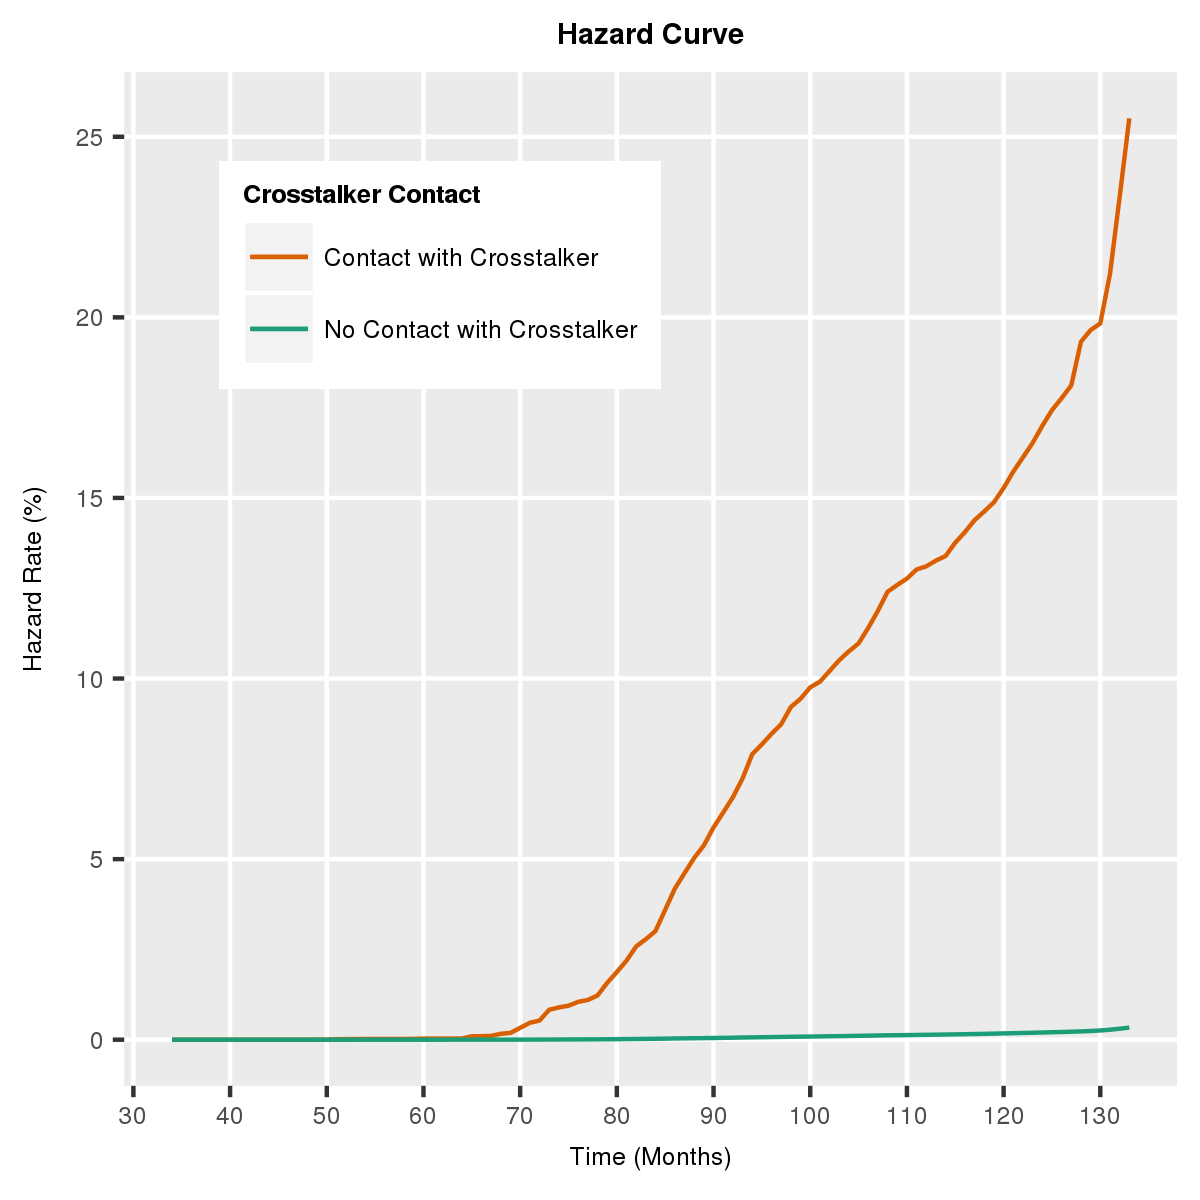
\includegraphics[scale=0.75]{contact_Hazard_final}
    \caption{Contact Hazard Curve}
    \label{fig:ctc_haz}
\end{figure}

\begin{figure}[ht]{}
\centering
    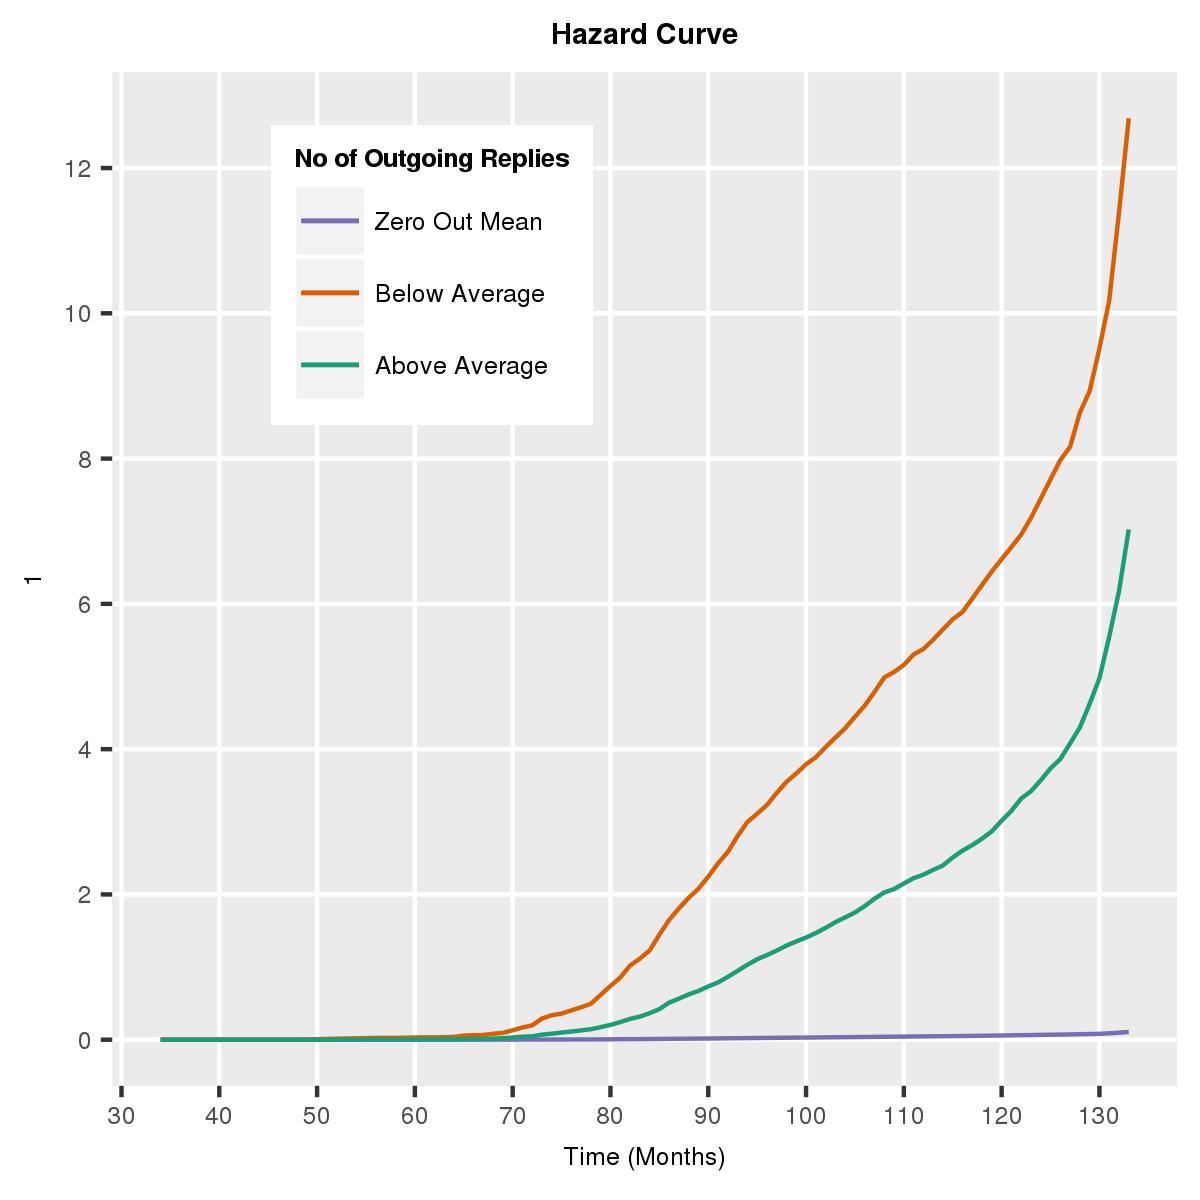
\includegraphics[scale=0.75]{outmean_Hazard_final}
    \caption{User Replies to Others Hazard Curve}
    \label{fig:outmean_haz}
\end{figure}
%In event history analysis, there are multiple methods for estimating the effects of the time-dependent co-variates. Here, we employ a Cox proportional hazards model, which estimates the effects of the independent variables on the rate at which cases move to a new state. The coefficients are interpreted as multiplicative effects on the hazard rate.

%\subsection{Results}
We begin with descriptive statistics. Figures~\ref{fig:bc_haz}-\ref{fig:outmean_haz} look at hazard curves \yy{precise definition needed} calculated for the entire sample. Overall, we find that only 8\% of all users in the Feminist and Men's Rights subreddits ever comment in the corresponding opposing group.\yy{this is already mentioned above, and it is not new information from the hazard curve} Figure~\ref{fig:bc_haz} indicates that interaction between Men's Rights and Feminism authors is a relatively uncommon behavior. \yy{same. nothing new here} The hazard curves also show important variation between subreddits. We found that users who begin in /r/Feminism were much more likely to post in /r/Men'sRights than the opposite.  Roughly speaking, /r/Feminist authors are 2.5 times as likely to cross the boundary into Men's Rights as their counterparts. \yy{no. without evidence that shows the community size difference does not matter, the following statement is not supported. there can be many null models that explain this without any difference in behavior but with pure size difference. } \del{This strongly suggests that these groups are highly heterogeneous. This may be due to selection effects or the norms that are adopted in the various groups regarding having discussions with others.}

\begin{table}
\caption{Descriptive Statistics and Correlations}
\centering
\begin{threeparttable}
\begin{adjustbox}{max width=\columnwidth}
\begin{tabular}{|c||r|r|r|r|r|}
\hline
& \multicolumn{5}{|c|}{\textbf{Descriptive Statistics}} \\\hline
\multicolumn{1}{|c||}{\textbf{Variable}}& \multicolumn{1}{l|}{\textbf{N}} & \multicolumn{1}{l|}{\textbf{mean}} & \multicolumn{1}{l|}{\textbf{sd}} & \multicolumn{1}{l|}{\textbf{min}} & \multicolumn{1}{l||}{\textbf{max}} \\\hline
Name Length & 4,605,955 & 10.7558 & 3.7168 & 3  & 20\\
First Cross-Talk & 4,605,955 & 0.0019 & 0.0437 & 0 & 1 \\
Wordiness& 4,605,955 & 3.5409 & 20.7327 & 0     & 1744 \\
Comments Written by User & 4,605,955 & 0.0379 & 0.1759 & 0 & 2 \\
Comments on User's Posts & 4,605,955 & 0.0402 & 0.2370 & 0 & 33 \\
Average Score & 4,605,955 & 0.3843 & 4.0352 & -266  & 1216 \\
Account Age & 4,302,176 & 1770.37 & 624.4882 & 1& 4021  \\
Feminism & 4,605,955 & 0.1512 & 0.3583 & 0  & 1 \\
Crossposter Talks to User & 4,605,955 & 0.0046 & 0.0675 & 0 & 1 \\
User Talks to Crossposter & 4,605,955 & 0.0044 & 0.0663 & 0  & 1\\
Difference between comments out and in & 4,605,955 & -0.0023 & 0.2071 & -33   & 2 \\\hline

\end{tabular}%
\end{adjustbox}
\end{threeparttable}
\label{tab:descrstat}
%\caption{\yy{sorry but the font size is way too small. We can't put a table like this. Same for the other tables. The all text in the table should be in legible size. maybe a couple of points (pt) smaller than the body text is fine. but no smaller than that.}}
\end{table}



\begin{table*}
\caption{Correlation Table}
\centering
\begin{threeparttable}
\begin{adjustbox}{max width=\textwidth}
\begin{tabular}{|p{4cm}||r|r|r|r|r|r|r|r|r|r|r|}
\hline
& \multicolumn{11}{c|}{\textbf{Correlations}} \\\hline
\multicolumn{1}{|c||}{\textbf{Variable}} & \multicolumn{1}{l|}{\textbf{Name Length}} & \multicolumn{1}{p{2cm}|}{\textbf{First Cross-Talk}} & \multicolumn{1}{l|}{\textbf{Wordiness}} & \multicolumn{1}{p{2cm}|}{\textbf{Comments Written by User}} & \multicolumn{1}{p{2cm}|}{\textbf{Comments on User's Posts}} & \multicolumn{1}{p{2cm}|}{\textbf{Average Score}} & \multicolumn{1}{p{2cm}|}{\textbf{Account Age}} & \multicolumn{1}{l|}{\textbf{Feminism}} & \multicolumn{1}{p{2cm}|}{\textbf{Crossposter Talks to User}} & \multicolumn{1}{p{2cm}|}{\textbf{User Talks to Crossposter}} & \multicolumn{1}{p{2cm}|}{\textbf{Difference between comments out and in}} \\\hline
Name Length & 1.0000 &  & &  &  &  & &  &  & & \\
First Cross-Talk & 0.0003 & 1.0000 & & & & & & & & &  \\
Wordiness& -0.0003 & 0.1119 & 1.0000 &  &  & &       &       &       &       &  \\
Comments Written by User & -0.0008 & 0.1207 & 0.4515 & 1.0000 & & & & & & &  \\
Comments on User's Posts & 0.0000 & 0.0909 & 0.4125 & 0.5287 & 1.0000 & & & & & &  \\
Average Score & -0.0010 & 0.0351 & 0.1991 & 0.2512 & 0.4260 & 1.0000 & & & & &  \\
Account Age & -0.2014 & -0.0105 & -0.0465 & -0.0586 & -0.0482 & -0.0273 & 1.0000 &       & & &  \\
Feminism & 0.0331 & 0.0233 & 0.0078 & -0.0215 & -0.0154 & -0.0059 & -0.1583 & 1.0000 & & &  \\
Crossposter Talks to User & -0.0009 & 0.1289 & 0.1859 & 0.2094 & 0.2428 & 0.0831 & -0.0109 & 0.0162 & 1.0000 & &  \\
User Talks to Crossposter & -0.0004 & 0.1294 & 0.1726 & 0.2501 & 0.1624 & 0.0627 & -0.0104 & 0.0158 & 0.6140 & 1.0000 &  \\
Difference between comments out and in & -0.0007 & -0.0018 & -0.0894 & 0.2419 & -0.6957 & -0.2743 & 0.0055 & -0.0006 & -0.1003 & 0.0260 & 1.0000 \\\hline

\end{tabular}%
\end{adjustbox}
\end{threeparttable}
\label{tab:descrstatcorr}
%\caption{\yy{sorry but the font size is way too small. We can't put a table like this. Same for the other tables. The all text in the table should be in legible size. maybe a couple of points (pt) smaller than the body text is fine. but no smaller than that.}}
\end{table*}


%Similarly, Figure \ref{fig:outmean_haz} shows modest differences between \del{users} \pat{authors} who have an above average number of replies to others' posts are much more likely to become \del{cross posters} \pat{boundary crossers}. Together, these hazard models suggest that openness and contact with boundary crossers are associated with boundary crossing.

Table~\ref{tab:regrtab} reports a series of models that independently, then jointly, test the hypotheses about the effects of different aspects of online behavior on boundary crossing. In many cases, our measures of the volume of online participation have positive and significant effects, yet they are small in size. For example, in Models 1 and 2, the effect of the average number of words per post is small ($0.005$). Thus, it would take hundreds of words per post to generate a large effect according to this model. Similar things can be said about the other variables in this table. The effects are small, though statistically significant.

The next table shows a much stronger effect for having an interaction with other users who are already cross-posting. Depending on the direction of the communication, the effect of having an interaction with a cross-poster is roughly 4.6 and reduces to 3.3 with the inclusion of control variables (see Models 9-12). This is larger than nearly every other variable with a significant effect included in the model.

Table 6 shows the full model with all independent variables and control variables included. In this model, many of the variables are still significant but the control variables have reduced the size of the main effects. In this model, contact with cross-posters, both to and from, has a significant effect but it is much attenuated. The variable of interest with the largest effect is the number of comments written by the user ($2.98$). 

These tables suggest the following about the relationship between the intensity of online interactions and cross-posting or cross-talk across these two online communities. First, there is a modest effect of the intensity and frequency of interaction on the initiation of outgroup interaction. Second, the largest effects tend to be associated with behavior where the user initiates the behavior. Talk to a cross-poster has a larger effect on cross-talk than being talke to by a cross-poster. A similar result was found for being the source and target of comments. Third, the control variables in Table 6 are either not significant or their estimated is extremely small. This suggests that the differences between reddits and the differences over time that were discussed in the descriptive statistics should be attributed to changes in the number of users who dedicated participants in the reddits.

\yy{maybe good to extract each table to a separate file. easier to edit.}

\begin{table*}
\caption{Modelling User Activity on Cross-talk}
\centering
\begin{threeparttable}
\begin{adjustbox}{max width=\textwidth}
\begin{tabular}{|p{4cm}|c|cccc|cccc|cccc|cccc|cccc|cccc|}
\hline
\multicolumn{1}{|r|}{} &       & \multicolumn{4}{c|}{\textbf{Model 1}} & \multicolumn{4}{c|}{\textbf{Model 2}} & \multicolumn{4}{c|}{\textbf{Model 3}} & \multicolumn{4}{c|}{\textbf{Model 4}} & \multicolumn{4}{c|}{\textbf{Model 5}} & \multicolumn{4}{c|}{\textbf{Model 6}} \\\hline

\multicolumn{1}{|c|}{\textbf{Variable}} & \textbf{Value} & \multicolumn{1}{c|}{\textbf{coef}} & \multicolumn{1}{c|}{\textbf{z}} & \multicolumn{1}{c|}{\textbf{p-value}} & \textbf{sig} & \multicolumn{1}{c|}{\textbf{coef}} & \multicolumn{1}{c|}{\textbf{z}} & \multicolumn{1}{c|}{\textbf{p-value}} & \textbf{sig} & \multicolumn{1}{c|}{\textbf{coef}} & \multicolumn{1}{c|}{\textbf{z}} & \multicolumn{1}{c|}{\textbf{p-value}} & \textbf{sig} & \multicolumn{1}{c|}{\textbf{coef}} & \multicolumn{1}{c|}{\textbf{z}} & \multicolumn{1}{c|}{\textbf{p-value}} & \textbf{sig} & \multicolumn{1}{c|}{\textbf{coef}} & \multicolumn{1}{c|}{\textbf{z}} & \multicolumn{1}{c|}{\textbf{p-value}} & \textbf{sig} & \multicolumn{1}{c|}{\textbf{coef}} & \multicolumn{1}{c|}{\textbf{z}} & \multicolumn{1}{c|}{\textbf{p-value}} & \textbf{sig} \\\hline

Wordiness &       & \multicolumn{1}{r|}{0.0060} & \multicolumn{1}{r|}{148.8} & \multicolumn{1}{r|}{\textless2e-16} & \multicolumn{1}{r|}{***} & \multicolumn{1}{r|}{0.0053} & \multicolumn{1}{r|}{110.506} & \multicolumn{1}{r|}{\textless2e-16} & \multicolumn{1}{r|}{***} & \multicolumn{1}{r|}{} & \multicolumn{1}{r|}{} & \multicolumn{1}{r|}{} &       & \multicolumn{1}{r|}{} & \multicolumn{1}{r|}{} & \multicolumn{1}{r|}{} &       & \multicolumn{1}{r|}{} & \multicolumn{1}{r|}{} & \multicolumn{1}{r|}{} &       & \multicolumn{1}{r|}{} & \multicolumn{1}{r|}{} & \multicolumn{1}{r|}{} &  \\
Comments on User's Posts &       & \multicolumn{1}{r|}{} & \multicolumn{1}{r|}{} & \multicolumn{1}{r|}{} &       & \multicolumn{1}{r|}{} & \multicolumn{1}{r|}{} & \multicolumn{1}{r|}{} &       & \multicolumn{1}{r|}{0.3307} & \multicolumn{1}{r|}{121.1} & \multicolumn{1}{r|}{\textless2e-16} & \multicolumn{1}{l|}{***} & \multicolumn{1}{r|}{0.3532} & \multicolumn{1}{r|}{90.617} & \multicolumn{1}{r|}{\textless2e-16} & \multicolumn{1}{l|}{***} & \multicolumn{1}{r|}{} & \multicolumn{1}{r|}{} & \multicolumn{1}{r|}{} &       & \multicolumn{1}{r|}{} & \multicolumn{1}{r|}{} & \multicolumn{1}{r|}{} &  \\
Comments Written by User &       & \multicolumn{1}{r|}{} & \multicolumn{1}{r|}{} & \multicolumn{1}{r|}{} &       & \multicolumn{1}{r|}{} & \multicolumn{1}{r|}{} & \multicolumn{1}{r|}{} &       & \multicolumn{1}{r|}{} & \multicolumn{1}{r|}{} & \multicolumn{1}{r|}{} &       & \multicolumn{1}{r|}{} & \multicolumn{1}{r|}{} & \multicolumn{1}{r|}{} &       & \multicolumn{1}{r|}{3.8596} & \multicolumn{1}{r|}{177.7} & \multicolumn{1}{r|}{\textless2e-16} & \multicolumn{1}{l|}{***} & \multicolumn{1}{r|}{3.559} & \multicolumn{1}{r|}{143.92} & \multicolumn{1}{r|}{\textless2e-16} & \multicolumn{1}{l|}{***} \\\hline

\textbf{Controls} &       & \multicolumn{1}{r|}{} & \multicolumn{1}{r|}{} & \multicolumn{1}{r|}{} &       & \multicolumn{1}{r|}{} & \multicolumn{1}{r|}{} & \multicolumn{1}{r|}{} &       & \multicolumn{1}{r|}{} & \multicolumn{1}{r|}{} & \multicolumn{1}{r|}{} &       & \multicolumn{1}{r|}{} & \multicolumn{1}{r|}{} & \multicolumn{1}{r|}{} &       & \multicolumn{1}{r|}{} & \multicolumn{1}{r|}{} & \multicolumn{1}{r|}{} &       & \multicolumn{1}{r|}{} & \multicolumn{1}{r|}{} & \multicolumn{1}{r|}{} &  \\\hline

Account age &       & \multicolumn{1}{r|}{} & \multicolumn{1}{r|}{} & \multicolumn{1}{r|}{} &       & \multicolumn{1}{r|}{-0.0009} & \multicolumn{1}{r|}{-34.102} & \multicolumn{1}{r|}{\textless2e-16} & \multicolumn{1}{r|}{***} & \multicolumn{1}{r|}{} & \multicolumn{1}{r|}{} & \multicolumn{1}{r|}{} &       & \multicolumn{1}{r|}{-0.0010} & \multicolumn{1}{r|}{-36.247} & \multicolumn{1}{r|}{\textless2e-16} & \multicolumn{1}{r|}{***} & \multicolumn{1}{r|}{} & \multicolumn{1}{r|}{} & \multicolumn{1}{r|}{} &       & \multicolumn{1}{r|}{-0.0004} & \multicolumn{1}{r|}{-17.445} & \multicolumn{1}{r|}{\textless2e-16} & \multicolumn{1}{r|}{***} \\
Name Length &       & \multicolumn{1}{r|}{} & \multicolumn{1}{r|}{} & \multicolumn{1}{r|}{} &       & \multicolumn{1}{r|}{-0.0157} & \multicolumn{1}{r|}{-5.115} & \multicolumn{1}{r|}{3.13e-07} & \multicolumn{1}{r|}{***} & \multicolumn{1}{r|}{} & \multicolumn{1}{r|}{} & \multicolumn{1}{r|}{} &       & \multicolumn{1}{r|}{-0.0172} & \multicolumn{1}{r|}{-5.606} & \multicolumn{1}{r|}{2.07e-08} & \multicolumn{1}{r|}{***} & \multicolumn{1}{r|}{} & \multicolumn{1}{r|}{} & \multicolumn{1}{r|}{} &       & \multicolumn{1}{r|}{-0.0106} & \multicolumn{1}{r|}{-3.456} & \multicolumn{1}{r|}{0.0005} & \multicolumn{1}{r|}{***} \\
Feminism &       & \multicolumn{1}{r|}{} & \multicolumn{1}{r|}{} & \multicolumn{1}{r|}{} &       & \multicolumn{1}{r|}{1.003} & \multicolumn{1}{r|}{41.491} & \multicolumn{1}{r|}{\textless2e-16} & \multicolumn{1}{r|}{***} & \multicolumn{1}{r|}{} & \multicolumn{1}{r|}{} & \multicolumn{1}{r|}{} &       & \multicolumn{1}{r|}{1.068} & \multicolumn{1}{r|}{44.17} & \multicolumn{1}{r|}{\textless2e-16} & \multicolumn{1}{r|}{***} & \multicolumn{1}{r|}{} & \multicolumn{1}{r|}{} & \multicolumn{1}{r|}{} &       & \multicolumn{1}{r|}{1.194} & \multicolumn{1}{r|}{49.991} & \multicolumn{1}{r|}{\textless2e-16} & \multicolumn{1}{r|}{***} \\
Average Score &       & \multicolumn{1}{r|}{} & \multicolumn{1}{r|}{} & \multicolumn{1}{r|}{} &       & \multicolumn{1}{r|}{0.0062} & \multicolumn{1}{r|}{25.161} & \multicolumn{1}{r|}{\textless2e-16} & \multicolumn{1}{r|}{***} & \multicolumn{1}{r|}{} & \multicolumn{1}{r|}{} & \multicolumn{1}{r|}{} &       & \multicolumn{1}{r|}{0.0009} & \multicolumn{1}{r|}{2.481} & \multicolumn{1}{r|}{0.0131} & \multicolumn{1}{r|}{*} & \multicolumn{1}{r|}{} & \multicolumn{1}{r|}{} & \multicolumn{1}{r|}{} &       & \multicolumn{1}{r|}{0.0048} & \multicolumn{1}{r|}{9.34} & \multicolumn{1}{r|}{\textless2e-16} & \multicolumn{1}{r|}{***} \\
2010 & \multicolumn{1}{l|}{\textbf{TRUE}} & \multicolumn{1}{r|}{} & \multicolumn{1}{r|}{} & \multicolumn{1}{r|}{} &       & \multicolumn{1}{r|}{12.73} & \multicolumn{1}{r|}{0.631} & \multicolumn{1}{r|}{0.5281} &       & \multicolumn{1}{r|}{} & \multicolumn{1}{r|}{} & \multicolumn{1}{r|}{} &       & \multicolumn{1}{r|}{99.12} & \multicolumn{1}{r|}{Inf} & \multicolumn{1}{r|}{\textless2e-16} & \multicolumn{1}{r|}{***} & \multicolumn{1}{r|}{} & \multicolumn{1}{r|}{} & \multicolumn{1}{r|}{} &       & \multicolumn{1}{r|}{31.8} & \multicolumn{1}{r|}{Inf} & \multicolumn{1}{r|}{\textless2e-16} & \multicolumn{1}{r|}{***} \\
2011 & \multicolumn{1}{l|}{\textbf{TRUE}} & \multicolumn{1}{r|}{} & \multicolumn{1}{r|}{} & \multicolumn{1}{r|}{} &       & \multicolumn{1}{r|}{12.51} & \multicolumn{1}{r|}{1.701} & \multicolumn{1}{r|}{0.0890} &       & \multicolumn{1}{r|}{} & \multicolumn{1}{r|}{} & \multicolumn{1}{r|}{} &       & \multicolumn{1}{r|}{17.98} & \multicolumn{1}{r|}{0.158} & \multicolumn{1}{r|}{0.8746} &       & \multicolumn{1}{r|}{} & \multicolumn{1}{r|}{} & \multicolumn{1}{r|}{} &       & \multicolumn{1}{r|}{23.8} & \multicolumn{1}{r|}{0.011} & \multicolumn{1}{r|}{0.9909} &  \\
2012 & \multicolumn{1}{l|}{\textbf{TRUE}} & \multicolumn{1}{r|}{} & \multicolumn{1}{r|}{} & \multicolumn{1}{r|}{} &       & \multicolumn{1}{r|}{12.42} & \multicolumn{1}{r|}{2.816} & \multicolumn{1}{r|}{0.0049} & \multicolumn{1}{r|}{**} & \multicolumn{1}{r|}{} & \multicolumn{1}{r|}{} & \multicolumn{1}{r|}{} &       & \multicolumn{1}{r|}{15.43} & \multicolumn{1}{r|}{0.774} & \multicolumn{1}{r|}{0.4391} &       & \multicolumn{1}{r|}{} & \multicolumn{1}{r|}{} & \multicolumn{1}{r|}{} &       & \multicolumn{1}{r|}{16.09} & \multicolumn{1}{r|}{0.507} & \multicolumn{1}{r|}{0.6125} &  \\
2013 & \multicolumn{1}{l|}{\textbf{TRUE}} & \multicolumn{1}{r|}{} & \multicolumn{1}{r|}{} & \multicolumn{1}{r|}{} &       & \multicolumn{1}{r|}{11.18} & \multicolumn{1}{r|}{3.65} & \multicolumn{1}{r|}{0.0003} & \multicolumn{1}{r|}{***} & \multicolumn{1}{r|}{} & \multicolumn{1}{r|}{} & \multicolumn{1}{r|}{} &       & \multicolumn{1}{r|}{16.76} & \multicolumn{1}{r|}{0.342} & \multicolumn{1}{r|}{0.7326} &       & \multicolumn{1}{r|}{} & \multicolumn{1}{r|}{} & \multicolumn{1}{r|}{} &       & \multicolumn{1}{r|}{15.29} & \multicolumn{1}{r|}{0.6} & \multicolumn{1}{r|}{0.5484} &  \\
2014 & \multicolumn{1}{l|}{\textbf{TRUE}} & \multicolumn{1}{r|}{} & \multicolumn{1}{r|}{} & \multicolumn{1}{r|}{} &       & \multicolumn{1}{r|}{10.56} & \multicolumn{1}{r|}{3.74} & \multicolumn{1}{r|}{0.0002} & \multicolumn{1}{r|}{***} & \multicolumn{1}{r|}{} & \multicolumn{1}{r|}{} & \multicolumn{1}{r|}{} &       & \multicolumn{1}{r|}{15.24} & \multicolumn{1}{r|}{0.564} & \multicolumn{1}{r|}{0.5725} &       & \multicolumn{1}{r|}{} & \multicolumn{1}{r|}{} & \multicolumn{1}{r|}{} &       & \multicolumn{1}{r|}{14.88} & \multicolumn{1}{r|}{0.604} & \multicolumn{1}{r|}{0.5462} &  \\
2015 & \multicolumn{1}{l|}{\textbf{TRUE}} & \multicolumn{1}{r|}{} & \multicolumn{1}{r|}{} & \multicolumn{1}{r|}{} &       & \multicolumn{1}{r|}{10.08} & \multicolumn{1}{r|}{2.965} & \multicolumn{1}{r|}{0.0030} & \multicolumn{1}{r|}{**} & \multicolumn{1}{r|}{} & \multicolumn{1}{r|}{} & \multicolumn{1}{r|}{} &       & \multicolumn{1}{r|}{16.22} & \multicolumn{1}{r|}{0.22} & \multicolumn{1}{r|}{0.8257} &       & \multicolumn{1}{r|}{} & \multicolumn{1}{r|}{} & \multicolumn{1}{r|}{} &       & \multicolumn{1}{r|}{19.8} & \multicolumn{1}{r|}{0.043} & \multicolumn{1}{r|}{0.9655} &  \\\hline

Number of User Months &       & \multicolumn{4}{c|}{\textbf{4,605,955}} & \multicolumn{4}{c|}{\textbf{4,605,955}} & \multicolumn{4}{c|}{\textbf{4,605,955}} & \multicolumn{4}{c|}{\textbf{4,605,955}} & \multicolumn{4}{c|}{\textbf{4,605,955}} & \multicolumn{4}{c|}{\textbf{4,605,955}} \\\hline
Authors who interact with outgroup &       & \multicolumn{4}{c|}{\textbf{8,816}} & \multicolumn{4}{c|}{\textbf{8,021}} & \multicolumn{4}{c|}{\textbf{8,816}} & \multicolumn{4}{c|}{\textbf{8,021}} & \multicolumn{4}{c|}{\textbf{8,816}} & \multicolumn{4}{c|}{\textbf{8,021}} \\\hline
Missing Observations &       & \multicolumn{4}{c|}{\textbf{0}} & \multicolumn{4}{c|}{\textbf{303,779}} & \multicolumn{4}{c|}{\textbf{0}} & \multicolumn{4}{c|}{\textbf{303,779}} & \multicolumn{4}{c|}{\textbf{0}} & \multicolumn{4}{c|}{\textbf{303,779}} \\\hline
$R^2$ &       & \multicolumn{4}{c|}{\textbf{0.001}} & \multicolumn{4}{c|}{\textbf{0.01}} & \multicolumn{4}{c|}{\textbf{0.001}} & \multicolumn{4}{c|}{\textbf{0.001}} & \multicolumn{4}{c|}{\textbf{0.005}} & \multicolumn{4}{c|}{\textbf{0.013}} \\\hline
Chis-squared Value &       & \multicolumn{4}{c|}{\textbf{4890}} & \multicolumn{4}{c|}{\textbf{42570}} & \multicolumn{4}{c|}{\textbf{2613}} & \multicolumn{4}{c|}{\textbf{41183}} & \multicolumn{4}{c|}{\textbf{22339}} & \multicolumn{4}{c|}{\textbf{55725}} \\\hline

\multicolumn{3}{l}{notes: * $p \leq 0.05$ ; ** $p \leq 0.01$ ; *** $p \leq 0.001$}{}&
\multicolumn{5}{l}{}&
\multicolumn{5}{l}{}&
\multicolumn{5}{l}{}\\
\end{tabular}
\end{adjustbox}
\end{threeparttable}
\label{tab:regrtab}
\end{table*}

\begin{table*}
\caption{Modelling Contact with Other Users on Cross-talk}
\centering
\begin{threeparttable}
 \begin{adjustbox}{max width=\textwidth}
                \begin{tabular}{|p{3.75cm}|c|cccc|cccc|cccc|cccc|cccc|cccc|}\hline
    \multicolumn{1}{|r|}{} &       & \multicolumn{4}{c|}{\textbf{Model 7}} & \multicolumn{4}{c|}{\textbf{Model 8}} & \multicolumn{4}{c|}{\textbf{Model 9}} & \multicolumn{4}{c|}{\textbf{Model 10}} & \multicolumn{4}{c|}{\textbf{Model 11}} & \multicolumn{4}{c|}{\textbf{Model 12}} \\\hline
    \textbf{Variable} & \multicolumn{1}{l|}{\textbf{Value}} & \multicolumn{1}{l|}{\textbf{coef}} & \multicolumn{1}{l|}{\textbf{z}} & \multicolumn{1}{l|}{\textbf{p-value}} & \multicolumn{1}{l|}{\textbf{sig}} & \multicolumn{1}{l|}{\textbf{coef}} & \multicolumn{1}{l|}{\textbf{z}} & \multicolumn{1}{l|}{\textbf{p-value}} & \multicolumn{1}{l|}{\textbf{sig}} & \multicolumn{1}{l|}{\textbf{coef}} & \multicolumn{1}{l|}{\textbf{z}} & \multicolumn{1}{l|}{\textbf{p-value}} & \multicolumn{1}{l|}{\textbf{sig}} & \multicolumn{1}{l|}{\textbf{coef}} & \multicolumn{1}{l|}{\textbf{z}} & \multicolumn{1}{l|}{\textbf{p-value}} & \multicolumn{1}{l|}{\textbf{sig}} & \multicolumn{1}{l|}{\textbf{coef}} & \multicolumn{1}{l|}{\textbf{z}} & \multicolumn{1}{l|}{\textbf{p-value}} & \multicolumn{1}{l|}{\textbf{sig}} & \multicolumn{1}{l|}{\textbf{coef}} & \multicolumn{1}{l|}{\textbf{z}} & \multicolumn{1}{l|}{\textbf{p-value}} & \multicolumn{1}{l|}{\textbf{sig}} \\\hline
    Difference between comments out and in &       & \multicolumn{1}{r|}{-0.1624} & \multicolumn{1}{r|}{-5.53} & \multicolumn{1}{r|}{3.3e-08} & \multicolumn{1}{r|}{***} & \multicolumn{1}{r|}{0.1826} & \multicolumn{1}{r|}{4.461} & \multicolumn{1}{r|}{8.2e-06} & \multicolumn{1}{r|}{***} & \multicolumn{1}{r|}{} & \multicolumn{1}{r|}{} & \multicolumn{1}{r|}{} &       & \multicolumn{1}{r|}{} & \multicolumn{1}{r|}{} & \multicolumn{1}{r|}{} &       & \multicolumn{1}{r|}{} & \multicolumn{1}{r|}{} & \multicolumn{1}{r|}{} &       & \multicolumn{1}{r|}{} & \multicolumn{1}{r|}{} & \multicolumn{1}{r|}{} &  \\
    Crossposter Talks to User & \multicolumn{1}{l|}{TRUE} & \multicolumn{1}{r|}{} & \multicolumn{1}{r|}{} & \multicolumn{1}{r|}{} &       & \multicolumn{1}{r|}{} & \multicolumn{1}{r|}{} & \multicolumn{1}{r|}{} &       & \multicolumn{1}{r|}{4.6017} & \multicolumn{1}{r|}{172.7} & \multicolumn{1}{r|}{\textless2e-16} & \multicolumn{1}{l|}{***} & \multicolumn{1}{r|}{3.321} & \multicolumn{1}{r|}{109.73} & \multicolumn{1}{r|}{\textless2e-16} & \multicolumn{1}{l|}{***} & \multicolumn{1}{r|}{} & \multicolumn{1}{r|}{} & \multicolumn{1}{r|}{} &       & \multicolumn{1}{r|}{} & \multicolumn{1}{r|}{} & \multicolumn{1}{r|}{} &  \\
    User Talks to Crossposter & \multicolumn{1}{l|}{TRUE} & \multicolumn{1}{r|}{} & \multicolumn{1}{r|}{} & \multicolumn{1}{r|}{} &       & \multicolumn{1}{r|}{} & \multicolumn{1}{r|}{} & \multicolumn{1}{r|}{} &       & \multicolumn{1}{r|}{} & \multicolumn{1}{r|}{} & \multicolumn{1}{r|}{} &       & \multicolumn{1}{r|}{} & \multicolumn{1}{r|}{} & \multicolumn{1}{r|}{} &       & \multicolumn{1}{r|}{4.6121} & \multicolumn{1}{r|}{172.2} & \multicolumn{1}{r|}{\textless2e-16} & \multicolumn{1}{l|}{***} & \multicolumn{1}{r|}{3.366} & \multicolumn{1}{r|}{111.77} & \multicolumn{1}{r|}{\textless2e-16} & \multicolumn{1}{l|}{***} \\\hline
    \textbf{Controls} &       & \multicolumn{1}{r|}{} & \multicolumn{1}{r|}{} & \multicolumn{1}{r|}{} &       & \multicolumn{1}{r|}{} & \multicolumn{1}{r|}{} & \multicolumn{1}{r|}{} &       & \multicolumn{1}{r|}{} & \multicolumn{1}{r|}{} & \multicolumn{1}{r|}{} &       & \multicolumn{1}{r|}{} & \multicolumn{1}{r|}{} & \multicolumn{1}{r|}{} &       & \multicolumn{1}{r|}{} & \multicolumn{1}{r|}{} & \multicolumn{1}{r|}{} &       & \multicolumn{1}{r|}{} & \multicolumn{1}{r|}{} & \multicolumn{1}{r|}{} &  \\\hline
    Account age &       & \multicolumn{1}{r|}{} & \multicolumn{1}{r|}{} & \multicolumn{1}{r|}{} &       & \multicolumn{1}{r|}{-0.0011} & \multicolumn{1}{r|}{-39.209} & \multicolumn{1}{r|}{\textless2e-16} & \multicolumn{1}{r|}{***} & \multicolumn{1}{r|}{} & \multicolumn{1}{r|}{} & \multicolumn{1}{r|}{} &       & \multicolumn{1}{r|}{-0.0008} & \multicolumn{1}{r|}{-30.697} & \multicolumn{1}{r|}{\textless2e-16} & \multicolumn{1}{r|}{***} & \multicolumn{1}{r|}{} & \multicolumn{1}{r|}{} & \multicolumn{1}{r|}{} &       & \multicolumn{1}{r|}{-0.0008} & \multicolumn{1}{r|}{-31.128} & \multicolumn{1}{r|}{\textless2e-16} & \multicolumn{1}{r|}{***} \\
    Name Length &       & \multicolumn{1}{r|}{} & \multicolumn{1}{r|}{} & \multicolumn{1}{r|}{} &       & \multicolumn{1}{r|}{-0.0197} & \multicolumn{1}{r|}{-6.459} & \multicolumn{1}{r|}{1.06e-10} & \multicolumn{1}{r|}{***} & \multicolumn{1}{r|}{} & \multicolumn{1}{r|}{} & \multicolumn{1}{r|}{} &       & \multicolumn{1}{r|}{-0.0160} & \multicolumn{1}{r|}{-5.226} & \multicolumn{1}{r|}{1.74e-07} & \multicolumn{1}{r|}{***} & \multicolumn{1}{r|}{} & \multicolumn{1}{r|}{} & \multicolumn{1}{r|}{} &       & \multicolumn{1}{r|}{-0.0172} & \multicolumn{1}{r|}{-5.623} & \multicolumn{1}{r|}{1.88e-08} & \multicolumn{1}{r|}{***} \\
    Feminism &       & \multicolumn{1}{r|}{} & \multicolumn{1}{r|}{} & \multicolumn{1}{r|}{} &       & \multicolumn{1}{r|}{1.031} & \multicolumn{1}{r|}{42.84} & \multicolumn{1}{r|}{\textless2e-16} & \multicolumn{1}{r|}{***} & \multicolumn{1}{r|}{} & \multicolumn{1}{r|}{} & \multicolumn{1}{r|}{} &       & \multicolumn{1}{r|}{0.9174} & \multicolumn{1}{r|}{38.095} & \multicolumn{1}{r|}{\textless2e-16} & \multicolumn{1}{r|}{***} & \multicolumn{1}{r|}{} & \multicolumn{1}{r|}{} & \multicolumn{1}{r|}{} &       & \multicolumn{1}{r|}{0.9217} & \multicolumn{1}{r|}{38.289} & \multicolumn{1}{r|}{\textless2e-16} & \multicolumn{1}{r|}{***} \\
    Average Score &       & \multicolumn{1}{r|}{} & \multicolumn{1}{r|}{} & \multicolumn{1}{r|}{} &       & \multicolumn{1}{r|}{0.0084} & \multicolumn{1}{r|}{31.146} & \multicolumn{1}{r|}{\textless2e-16} & \multicolumn{1}{r|}{***} & \multicolumn{1}{r|}{} & \multicolumn{1}{r|}{} & \multicolumn{1}{r|}{} &       & \multicolumn{1}{r|}{0.0051} & \multicolumn{1}{r|}{21.762} & \multicolumn{1}{r|}{\textless2e-16} & \multicolumn{1}{r|}{***} & \multicolumn{1}{r|}{} & \multicolumn{1}{r|}{} & \multicolumn{1}{r|}{} &       & \multicolumn{1}{r|}{0.0073} & \multicolumn{1}{r|}{32.957} & \multicolumn{1}{r|}{\textless2e-16} & \multicolumn{1}{r|}{***} \\
    2010 & \multicolumn{1}{l|}{\textbf{TRUE}} & \multicolumn{1}{r|}{} & \multicolumn{1}{r|}{} & \multicolumn{1}{r|}{} &       & \multicolumn{1}{r|}{88.4} & \multicolumn{1}{r|}{Inf} & \multicolumn{1}{r|}{\textless2e-16} & \multicolumn{1}{r|}{***} & \multicolumn{1}{r|}{} & \multicolumn{1}{r|}{} & \multicolumn{1}{r|}{} &       & \multicolumn{1}{r|}{17.47} & \multicolumn{1}{r|}{0.086} & \multicolumn{1}{r|}{0.932} &       & \multicolumn{1}{r|}{} & \multicolumn{1}{r|}{} & \multicolumn{1}{r|}{} &       & \multicolumn{1}{r|}{17.39} & \multicolumn{1}{r|}{0.088} & \multicolumn{1}{r|}{0.93} &  \\
    2011 & \multicolumn{1}{l|}{\textbf{TRUE}} & \multicolumn{1}{r|}{} & \multicolumn{1}{r|}{} & \multicolumn{1}{r|}{} &       & \multicolumn{1}{r|}{19.62} & \multicolumn{1}{r|}{0.076} & \multicolumn{1}{r|}{0.9390} &       & \multicolumn{1}{r|}{} & \multicolumn{1}{r|}{} & \multicolumn{1}{r|}{} &       & \multicolumn{1}{r|}{18.26} & \multicolumn{1}{r|}{0.143} & \multicolumn{1}{r|}{0.886} &       & \multicolumn{1}{r|}{} & \multicolumn{1}{r|}{} & \multicolumn{1}{r|}{} &       & \multicolumn{1}{r|}{18.33} & \multicolumn{1}{r|}{0.14} & \multicolumn{1}{r|}{0.8880} &  \\
    2012 & \multicolumn{1}{l|}{\textbf{TRUE}} & \multicolumn{1}{r|}{} & \multicolumn{1}{r|}{} & \multicolumn{1}{r|}{} &       & \multicolumn{1}{r|}{19.5} & \multicolumn{1}{r|}{0.128} & \multicolumn{1}{r|}{0.8980} &       & \multicolumn{1}{r|}{} & \multicolumn{1}{r|}{} & \multicolumn{1}{r|}{} &       & \multicolumn{1}{r|}{17.49} & \multicolumn{1}{r|}{0.275} & \multicolumn{1}{r|}{0.784} &       & \multicolumn{1}{r|}{} & \multicolumn{1}{r|}{} & \multicolumn{1}{r|}{} &       & \multicolumn{1}{r|}{17.42} & \multicolumn{1}{r|}{0.287} & \multicolumn{1}{r|}{0.7740} &  \\
    2013 & \multicolumn{1}{l|}{\textbf{TRUE}} & \multicolumn{1}{r|}{} & \multicolumn{1}{r|}{} & \multicolumn{1}{r|}{} &       & \multicolumn{1}{r|}{15.37} & \multicolumn{1}{r|}{0.63} & \multicolumn{1}{r|}{0.5280} &       & \multicolumn{1}{r|}{} & \multicolumn{1}{r|}{} & \multicolumn{1}{r|}{} &       & \multicolumn{1}{r|}{16.25} & \multicolumn{1}{r|}{0.413} & \multicolumn{1}{r|}{0.68} &       & \multicolumn{1}{r|}{} & \multicolumn{1}{r|}{} & \multicolumn{1}{r|}{} &       & \multicolumn{1}{r|}{16.18} & \multicolumn{1}{r|}{0.423} & \multicolumn{1}{r|}{0.6720} &  \\
    2014 & \multicolumn{1}{l|}{\textbf{TRUE}} & \multicolumn{1}{r|}{} & \multicolumn{1}{r|}{} & \multicolumn{1}{r|}{} &       & \multicolumn{1}{r|}{14.59} & \multicolumn{1}{r|}{0.7} & \multicolumn{1}{r|}{0.4840} &       & \multicolumn{1}{r|}{} & \multicolumn{1}{r|}{} & \multicolumn{1}{r|}{} &       & \multicolumn{1}{r|}{15.68} & \multicolumn{1}{r|}{0.422} & \multicolumn{1}{r|}{0.673} &       & \multicolumn{1}{r|}{} & \multicolumn{1}{r|}{} & \multicolumn{1}{r|}{} &       & \multicolumn{1}{r|}{15.56} & \multicolumn{1}{r|}{0.448} & \multicolumn{1}{r|}{0.6540} &  \\
    2015 & \multicolumn{1}{l|}{\textbf{TRUE}} & \multicolumn{1}{r|}{} & \multicolumn{1}{r|}{} & \multicolumn{1}{r|}{} &       & \multicolumn{1}{r|}{13.98} & \multicolumn{1}{r|}{0.591} & \multicolumn{1}{r|}{0.5540} &       & \multicolumn{1}{r|}{} & \multicolumn{1}{r|}{} & \multicolumn{1}{r|}{} &       & \multicolumn{1}{r|}{15.15} & \multicolumn{1}{r|}{0.354} & \multicolumn{1}{r|}{0.724} &       & \multicolumn{1}{r|}{} & \multicolumn{1}{r|}{} & \multicolumn{1}{r|}{} &       & \multicolumn{1}{r|}{15.08} & \multicolumn{1}{r|}{0.365} & \multicolumn{1}{r|}{0.7150} &  \\\hline
    Number of User Months &       & \multicolumn{4}{c|}{\textbf{4,605,955}} & \multicolumn{4}{c|}{\textbf{4,605,955}} & \multicolumn{4}{c|}{\textbf{4,605,955}} & \multicolumn{4}{c|}{\textbf{4,605,955}} & \multicolumn{4}{c|}{\textbf{4,605,955}} & \multicolumn{4}{c|}{\textbf{4,605,955}} \\\hline
    Authors who interact with outgroup &       & \multicolumn{4}{c|}{\textbf{8,816}} & \multicolumn{4}{c|}{\textbf{8,021}} & \multicolumn{4}{c|}{\textbf{8,816}} & \multicolumn{4}{c|}{\textbf{8,021}} & \multicolumn{4}{c|}{\textbf{8,816}} & \multicolumn{4}{c|}{\textbf{8,021}} \\\hline
    Missing Observations &       & \multicolumn{4}{c|}{\textbf{0}} & \multicolumn{4}{c|}{\textbf{303,779}} & \multicolumn{4}{c|}{\textbf{0}} & \multicolumn{4}{c|}{\textbf{303,779}} & \multicolumn{4}{c|}{\textbf{0}} & \multicolumn{4}{c|}{\textbf{303,779}} \\\hline
    $R^2$ &       & \multicolumn{4}{c|}{\textbf{0}} & \multicolumn{4}{c|}{\textbf{0.009}} & \multicolumn{4}{c|}{\textbf{0.003}} & \multicolumn{4}{c|}{\textbf{0.011}} & \multicolumn{4}{c|}{\textbf{0.003}} & \multicolumn{4}{c|}{\textbf{0.011}} \\\hline
    Chis-squared Value &       & \multicolumn{4}{c|}{\textbf{16.76}} & \multicolumn{4}{c|}{\textbf{39136}} & \multicolumn{4}{c|}{\textbf{12641}} & \multicolumn{4}{c|}{\textbf{46110}} & \multicolumn{4}{c|}{\textbf{12498}} & \multicolumn{4}{c|}{\textbf{46227}} \\\hline
    
\multicolumn{3}{l}{notes: * $p \leq 0.05$ ; ** $p \leq 0.01$ ; *** $p \leq 0.001$}{}&
\multicolumn{5}{l}{}&
\multicolumn{5}{l}{}&
\multicolumn{5}{l}{}\\
    \end{tabular}%

\end{adjustbox}
\end{threeparttable}
\label{tab:regrtab2}
\end{table*}


\begin{table}[htb]
\caption{Saturated Regression Model}
\centering
\begin{threeparttable}
 \begin{adjustbox}{max width=\columnwidth}
 \begin{tabular}{|p{4cm}|c|r|r|r|}
    \hline
          & \multicolumn{4}{c|}{\textbf{Controlled Saturated Model}} \\
    \hline
    \textbf{Variables} & \multicolumn{1}{l|}{\textbf{coef}} & \multicolumn{1}{l|}{\textbf{z}} & \multicolumn{1}{l|}{\textbf{p-value}} & \multicolumn{1}{l|}{\textbf{sig}} \\
    \hline
    Wordiness & \multicolumn{1}{r|}{0.004} & 44.55 & \textless2e-16 & *** \\
    Comments on User's Posts & \multicolumn{1}{r|}{0.208} & 18.82 & \textless2e-16 & *** \\
    Comments Written by User & \multicolumn{1}{r|}{2.98} & 105.11 & \textless2e-16 & *** \\
    Crossposter Talks to User & \multicolumn{1}{r|}{1.1} & 23.62 & \textless2e-16 & *** \\
    User Talks to Crossposter & \multicolumn{1}{r|}{0.746} & 16.11 & \textless2e-16 & *** \\\hline
    
    \textbf{Controls} &       &       &       &  \\\hline
    
    Account Age & \multicolumn{1}{r|}{-3e-04} & -14.37 & \textless2e-16 & *** \\
    Average Score & \multicolumn{1}{r|}{-1e-04} & -0.1  & 0.9222 &  \\
    Feminism & \multicolumn{1}{r|}{0.994} & 40.96 & \textless2e-16 & *** \\
    Name Length & \multicolumn{1}{r|}{-0.011} & -3.43 & 0.0006 & *** \\
    2010  & \multicolumn{1}{r|}{15.1} & 0.21  & 0.8372 &  \\
    2011  & \multicolumn{1}{r|}{14.9} & 0.63  & 0.5295 &  \\
    2012  & \multicolumn{1}{r|}{13.9} & 1.22  & 0.2211 &  \\
    2013  & \multicolumn{1}{r|}{13.1} & 1.47  & 0.142 &  \\
    2014  & \multicolumn{1}{r|}{12.8} & 1.47  & 0.1407 &  \\
    2015  & \multicolumn{1}{r|}{12.3} & 1.14  & 0.2527 &  \\\hline
    
    \textbf{Number of User Months} & \multicolumn{4}{c|}{4,605,955} \\\hline
    
    \textbf{Authors who interact
 with outgroup} & \multicolumn{4}{c|}{8,021} \\\hline
    
    \textbf{Missing Observations} & \multicolumn{4}{c|}{303,779} \\\hline
    
    \textbf{$R^2$} & \multicolumn{4}{c|}{0.013} \\\hline
    
    \textbf{Chis-squared Value} & \multicolumn{4}{c|}{57858} \\
    \hline
    \multicolumn{5}{l}{notes: * $p \leq 0.05$ ; ** $p \leq 0.01$ ; *** $p \leq 0.001$}{}\\
    \end{tabular}%

\end{adjustbox}
\end{threeparttable}
\label{tab:regrtab3}
\end{table}

\subsection{An Implication of Cross-talk Between Men's Rights and Feminism: Linguistic Drift}

Here, we examine one consequence of cross-talking or cross-posting across these two subreddits. We provide evidence that cross-posting is associated with linguistic drift. Users who cross-post in the opposing subreddit resemble less their ``native'' or home subreddit after they start addressing the opposite reddit. \yy{I think ``which posts?'' is important to clarify. Are we saying that user A's posts on the home subreddit drift after posting to the other subreddit? or user A's posts (across both subreddits)? The latter can be trivial. }  To study the linguistic similarity of Reddit users, we preprocessed the raw text of Reddit posts, where HTML and other markup tags were removed. Then, each post was tokenized into bigrams. 

In our first analysis, we investigated if the cross-posters' linguistic pattern in their home subreddit has manifested a significant change between the pre- and post-crossposting stage. As a comparison, we also considered the posts in the same subreddit that are from authors who never cross-posted. These posts were split into those that occurred in the first and second half of an author's lifespan.

\begin{table}
    \caption{Count of Sentences of Posts From Cross-posters and Non-crossposters.}
    \centering
    \begin{adjustbox}{max width=\columnwidth}
    
    \begin{tabular}{|l l| r r|}\hline
        & & Men'sRights & Feminism\\
        \hline
        \hline
        \multirow{2}{*}{\textbf{Cross-poster}}& ``Pre-crossposting'' & 820,850   & 77,460\\
            & ``Post-crossposting''  & 2,494,351 & 149,112\\
            \hline
        \multirow{2}{*}{\textbf{Non-Crossposter}}   & ``First half''      & 1,315,380 & 193,058\\
            & ``Second half''       & 1,391,906 & 242,324\\\hline
    \end{tabular}
    \label{lm:tab1}
    \end{adjustbox}
\end{table}

For each group, a fixed number (100,000) of sentences were bootstrapped (i.e. sampled with replacement) from the available text data (Table~\ref{lm:tab1}), and for each sentence a log-transformed probability score was computed using bigram language model (with the Stupid backoff smoothing~\cite{Brants07largelanguage}). The bigram model was trained on the text data from non-crossposters in the same subreddit (disjoint from those used in the test set), which contains the most posts compared to those from cross-posters, and represents the mainstream linguistic pattern of the subreddit. The total number of available sentences in the four groups from which the above test and training set were sampled are briefly summarized in Table~\ref{lm:tab1}.  

%Bigram model was trained using 150,000 sentences from ``First half'' and ``Second half'', respectively, and 100,000 sentences were bootstrapped from the remaining in each of the four groups as the test set.

As illustrated in Figure~\ref{lm:fig1_1}, the linguistic pattern of both cross-posters and non-crossposters appeared to have drifted away from the mainstream of their home subreddit, when comparing the average of the log-probability of sentences in the early stage (``Pre-crossposting'' and ``First half'') and late stage (``Post-crossposting'' and ``Second half'') of an author's lifespan. Notice that the linguistic pattern of Feminism-to-Men'sRights cross-posters has drifted to a much larger degree compared to the Feminism non-crossposters. To evaluate the statistical significance of the observed difference in Feminism as well as the counterpart in Men's Rights, the procedure of training and test set sampling and language model building was repeated a hundred times, and for each repetition the delta ($\Delta_{cp}$) between ``Post-crossposting'' and ``Pre-crossposting'', and the delta ($\Delta_{Ncp}$) between ``Second half'' and ``First half'' was computed. The average of $\Delta_{cp}$ and the average of $\Delta_{Ncp}$ over the hundred repetitions was computed (Figure ~\ref{lm:fig1_2}). We found that, for Feminism, the average of $\Delta{cp}$ (0.1149) was found to be statistically different (t-test, p-value$\simeq 0$) from that of $\Delta_{Ncp}$ (0.0182). However, for Men'sRights the means of two samples of delta (0.0325 and 0.0320) was not found to be statistically different (t-test, p-value=0.5524), which may suggest that Feminism-to-Men'sRights cross-posters \del{appeared to be more radical or aggressive}\yy{no evidence on the nature of the content} than the Men'sRights-to-Feminism cross-posters in terms of the change of linguistic patterns.

\begin{figure}[ht]
    \centering
    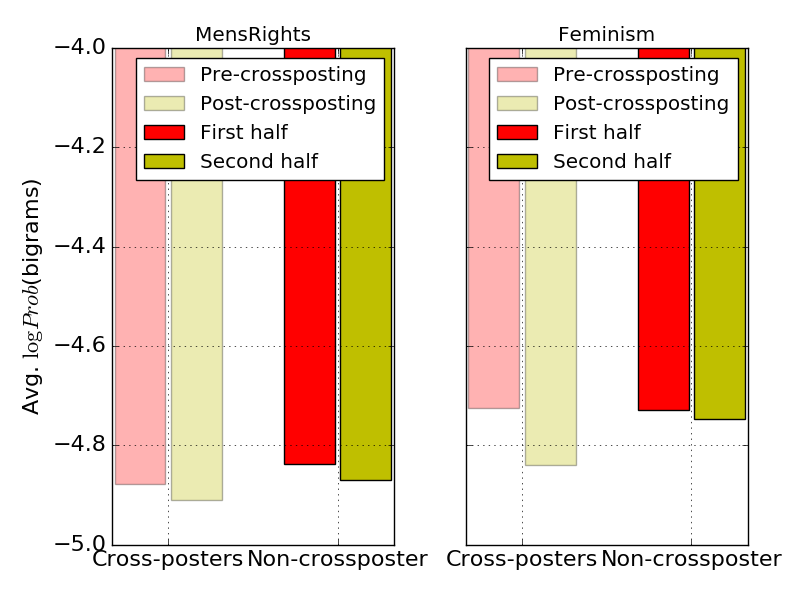
\includegraphics[scale = 0.4]{LM_figure_1_1}
    \caption{Change in Linguistic Pattern for Cross-posters and Non-crossposters.}
    \label{lm:fig1_1}
\end{figure}

\begin{figure}[ht]
    \centering
    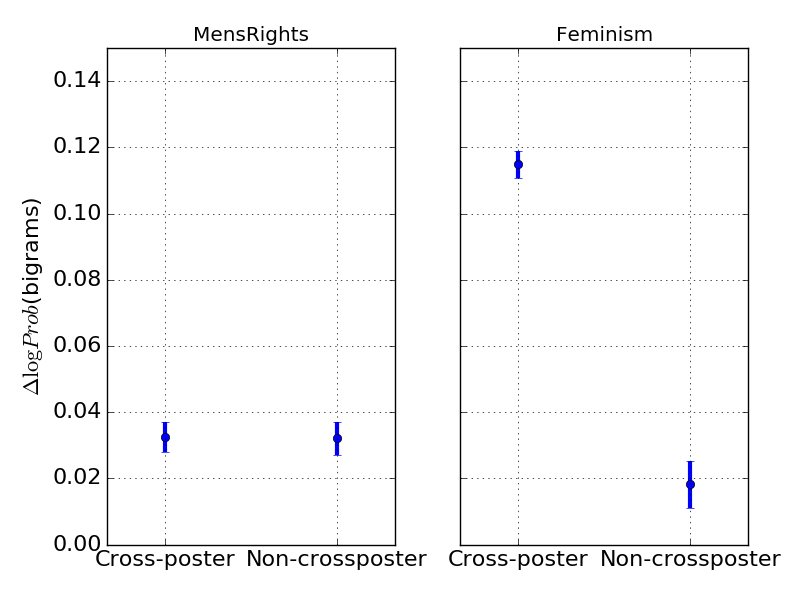
\includegraphics[scale = 0.4]{LM_figure_1_2}
    \caption{\yy{not sure what's being measured here} Feminism-to-Men'sRights Cross-posters appear to be different in Linguistic Pattern.}
    \label{lm:fig1_2}
\end{figure}

In the second analysis, we investigated whether the linguistic pattern of all authors (cross-posters and non-crossposters alike) has changed over the entire lifecycle of either subreddit. The posts were sorted in increasing order of the timestamp, and sorted list were split into 50 approximately equal-sized sub-samples. A log-probability was computed for each sentence in one portion of data, using a bigram model trained on the sentences from the remaining 49 samples, and this was repeated for each of the 50 data samples. As a comparison, we considered an irrelevant subreddit ``Cooking'' on which this process was repeated. We plotted the average of the log-probability of sentences in each sample as a function of the index (1 to 50). As shown in Figure XXX~\ref{lm:fig2}, the agreement of the local and the global linguistic pattern for both subreddits reached the maximum in the first half the lifecyle, and then decreases over time. In contrast, the linguistic pattern of the subreddit ``Cooking'' remains stable. It's also interesting to note that the evolution of the linguistic pattern in Men'sRights and Feminism appear to be correlated with each other ($\rho$ = 0.6636), in contrast to their correlation with the Cooking subreddit ($\rho$ = 0.3487 and 0.0445 for Men'sRights and Feminism). Taken together, these analyses of the language patterns of reddit users show that there are important consequence of cross-group contact.

\begin{figure}[ht]
    \centering
    \includegraphics[scale=0.4]{images/LM_figure_2.png}
    \label{lm:fig2}
    \caption{The Evolution of Linguistic Pattern over the Lifecyle of Subreddits}
\end{figure}

\subsection{Discussion}

We hypothesized that the tendency to address an ideologically opposite group was associated with wordiness, network degree and exposure to others who cross-post. Our data indicate that there is support most of these hypotheses. However, in many cases, the size of the effect is  small. The exception is the variable for having contact with others who cross-post. That has an  large effect. We noted earlier that there could be multiple explanations for this effect. There may be direct contagion or it may reflect homophily. If there is contagion, then further research can investigate the reasons why. For example, one possibility is that the user may learn about the ideologically opposite reddit through contact with a cross-poster. Alternatively, cross-talk may tend to be antagonistic. The appearance of cross-talkers may incite a user to visit the ideologically opposite reddit in an attempt to continue a dispute. 

It may also be the case that the spread of cross-talking or cross-posting behavior may be due to unobserved variables and not the contact with a cross-talker. For example, perhaps people with certain preferences for topics that overlap with Men's Rights and Feminism would naturally talk with each other. One issue might be the discussion of books that critique either Feminist or Men's Rights ideas from the other perspective. People who would be interested in such a debate might cross-post and comment on each other's text, even if they did not influence each other. Further research can assess whether the effects reported in this study are attributable to such unobserved variables.

The analysis of linguist drift shows that cross-talk between ideologically opposite groups might be an important component of cultural change. As individuals gain exposure to others from different ideological orientations, they may change the content of their speech. Although this does not mean that they adopt the opposite side's opinions, they may be changing in ways that shift the conversation within their own group.

\subsection{Conclusion} 

The main purpose of this study is to investigate the conditions under which individuals might choose to engage with a group that holds conflicting beliefs. Our evidence shows that a mixture of individual and structural factors are associated with this behavior. Our study of linguistic drift shows that cross-talking, in this case, leads to users who are substantively different in their discourse than their colleagues in their ``home'' subreddit. This drift might be one source of cultural and social change more generally. The exposure to outside groups leads to drift that, in some cases, may lead to a broader change in beliefs. By studying when cross-talk happens and some of the consequences, our research alludes to a larger account of how social boundaries, crossing, and linguistic change play a role in social change.

%\section{Discussion}
%[Fabio and Pat]
%We use the term \textit{crossposter} to describe those authors who interact with their ideological outgroup by posting in that subreddit, in this case,  /r/Men'sRights and /r/Feminism. Our hazard curves show that interactions between these two polarized subreddits continues throughout the nearly seven years of comment data for these subreddits, although there appear to be external factors of a temporal nature which affect the number of authors who emerge to interact as shown in figure \ref{fig:bc_yoe}. 

%\begin{figure}[htb]
    %\centering
    %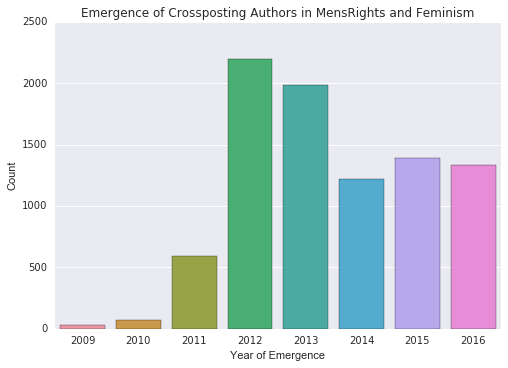
\includegraphics[scale=0.4]{bc_yr_of_emergence}
    %\caption{Crossposter Year of Emergence}
    %\label{fig:bc_yoe}
%\end{figure}

%\fxfatal{\pat{consistent use and spelling of Crossposter / Boundary Crosser}}
%Table \ref{tab:datasum} summarizes the comment data set and shows how the two subreddits differ by size with /r/Men'sRights being significantly larger in terms of numbers of authors and comments when compared to /r/Feminsim. Figure \ref{fig:bc_ratio} depicts the normalized count of comment authors by date of emergence and author type (/r/Men'sRights only, /r/Feminism only, and crossposter).  /r/Men'sRights authors are by far the largest count, followed by /r/Feminism authors and finally crossposters.  
%While we have not studied the cause of these (it is left for future work), we have been able to attribute several features relating to the author and how they post in their home subreddit as potential indicators. One particularly interesting finding is that the first subreddit in which an author posts is a good indicator of their potential to cross boundaries.  Consider the data in figure \ref{fig:bc_tot} where /r/Feminism contributes an appreciable number of boundary crossing authors given its relatively small size when compared with /r/Men'sRights.

%\begin{figure}[ht]
%    \centering
    %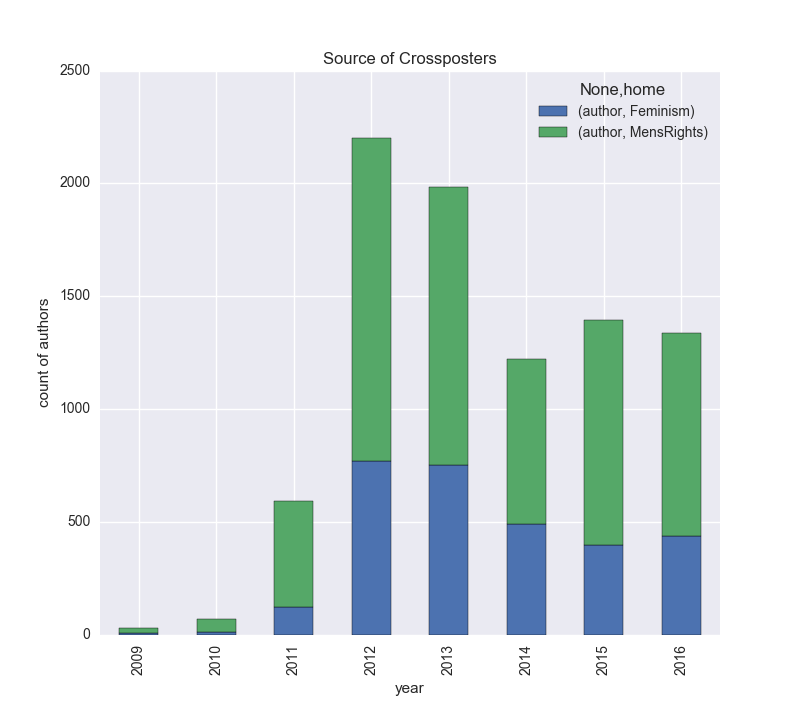
\includegraphics[scale=0.4]{tot_bc_count}
    %\caption{Boundary Crossers by Subreddit}
%    \label{fig:bc_tot}
%\end{figure}

%\subsection{Association between the act of cross-posting and the drift of linguistic pattern of cross-posters}
%Also of interest is our finding that an author's language changes after interacting with the opposite subreddit.Figure~\ref{fig:LMchange} depicts the language changes before and after crossposting for authors by their principal subreddit using a bigram language model which analyzes author comments.  Notice that the \pat{need some words from Chao Ji here...}

%The raw text of reddit posts (\texttt{body} field) were preprocessed, where HTML and other markup tags were removed. Then each post was tokenized into sentences, and each sentence was represented as a Bigram sequence of tokenized words. We performed two controlled computational experiments on the reddit text data processed as above using statistical language models.

%In the first experiment, we investigated if the cross-posters' linguistic pattern in their HOME subreddit has manifested a significant change between the pre- and post-crossposting stage. As a comparison, we also considered the posts in the same subreddit that are from authors who never cross-posted. These posts were split into those that occurred in the first and second half of an author's lifespan. 

%For each group, a fixed number (100,000) of sentences were bootstrapped (i.e. sampled with replacement) from the available text data (Table ~\ref{lm:tab1}), and for each sentence a log-transformed probability score was computed using Bigram language model (with Stupid backoff smoothing ~\cite{Brants07largelanguage}). The Bigram model was trained on the text data from non-crossposters in the same subreddit (disjoint from those used in the test set), which contains the most posts compared to those from cross-posters, and represents the mainstream linguistic pattern of the subreddit. The total numbers of available sentences in the four groups from which the above test and training set were sampled are briefly summarized in Table ~\ref{lm:tab1}. 

%As illustrated in Figure ~\ref{lm:fig1_1}, the linguistic pattern of both cross-posters and non-crossposters appeared to have drifted away from the mainstream of their HOME subreddit, when comparing the average of the log-probability of sentences in the early stage ("Pre-crossposting" and "First half") and late stage ("Post-crossposting" and "Second half") of an author's lifespan. Notice that the linguistic pattern of Feminism-to-Men'sRights cross-posters has drifted to a much larger degree compared to the Feminism non-crossposters. To evaluate the statistical significance of the observed difference in Feminism as well as the counterpart in Men'sRights, the procedure of training and test set sampling and language model building was repeated a hundred times, and for each repetition the delta ($\Delta_{cp}$) between "Post-crossposting" and "Pre-crossposting", and the delta ($\Delta_{Ncp}$) between "Second half" and "First half" was computed. The average of $\Delta_{cp}$ and the average of $\Delta_{Ncp}$ over the hundred repetitions was computed (Figure ~\ref{lm:fig1_2}). We found that, for Feminism, the average of $\Delta{cp}$ (0.1149) was found to be statistically different (t-test, p-value=$2.5e-184$) from that of $\Delta_{Ncp}$ (0.0182). However, for Men'sRights the means of two samples of delta (0.0325 and 0.0320) was not found to be statistically different (t-test, p-value=0.5524), which may suggest that Feminism-to-Men'sRights cross-posters appeared to be more radical or aggressive than the Men'sRights-to-Feminism cross-posters in terms of the change of linguistic patterns.

%We also analyzed the change in language used in /r/Men'sRights and /f/Feminism over time when compared to a less controversial subreddit, /r/Cooking.  \pat{write findings here}

%\begin{figure}[ht]
%    \centering
%    \includegraphics[scale=0.4]{LM_figure_2}
%    \caption{Changes in SR Language Over Time}
%    \label{fig:SRlangchanges}
%\end{figure}

%In the second experiment, we investigated whether the linguistic pattern of all authors (cross-posters and non-crossposters alike) has changed over the entire lifecycle of either subreddit. The posts were sorted in increasing order of the timestamp, and sorted list were split into 50 approximately equal-sized chunks. A log-probability was computed for each sentence in one chunk of data, using a Bigram model trained on the sentences from the remaining 49 chunks, and this was repeated for each of the 50 chunks. As a comparison, we considered an irrelevant subreddit "Cooking" on which this process was repeated. We plotted the average of the log-probability of sentences in each chunk as a function of the index (1 to 50). As shown in Figure ~\ref{lm:fig2}, for Men'sRights and Feminism the agreement of the local and the global linguistic pattern reached the maximum in the first half the lifecyle, and then decreases over time. In contrast, the linguistic pattern of the subreddit "Cooking" remains stable. It's also interesting to note that the evolution of the linguistic pattern in Men'sRights and Feminism appear to be correlated with each other ($\rho$ = 0.6636), in contrast to their correlation with the Cooking subreddit ($\rho$ = 0.3487 and 0.0445 for Men'sRights and Feminism). 



%\section{Conclusion}
%[Fabio]
%\%\%\%\%\%\%\%\%\%
% \textit{References and End of Paper}
\bibliographystyle{aaai}
\bibliography{refs.bib}
\end{document}